\documentclass[watermark,final]{thesis}  % draft mode (default)
%\documentclass[review]{thesis}  % review mode (show contents & reference only)
%\documentclass[watermark,final]{thesis}  % final mode (version for library)

%-------------------------------------------------------------------------------
% Package Loading
%-------------------------------------------------------------------------------

% font
\usepackage{fontspec}
\setmonofont[Scale=0.8]{Droid Sans Mono}

% spacing
\newcommand{\eqlineskip}{0.3\baselineskip}
\newcommand{\resultfigwidth}{0.78\textwidth}

% title format
\newcommand{\partopic}[1]{\noindent\textbf{#1}}

% math
\usepackage{amsmath,amssymb,amsfonts}
\usepackage{mathtools}
\DeclareMathOperator{\where}{\mid\,}
\DeclareMathOperator{\divby}{/}
\DeclareMathOperator{\avg}{avg}
\DeclareMathOperator{\precision}{precision}
\DeclareMathOperator{\recall}{recall}
\newcommand{\fscore}{F\textsubscript{1}-score}

% list
\usepackage{enumitem}
\setlist{nosep}

% table
\usepackage{array}
\usepackage{multirow}
\usepackage{tablefootnote}
\renewcommand{\arraystretch}{1.35}

% caption
\usepackage[font=small,labelfont=bf]{caption}
\usepackage{subcaption}
\newcommand{\tblskip}{3pt}
\captionsetup[table]{skip=\tblskip}
\captionsetup[subtable]{font=small,labelfont=bf,labelformat=parens,skip=\tblskip}

% footnote
\usepackage[bottom]{footmisc}


% draw
\usepackage{tikz}
\usetikzlibrary{positioning}

% box
\usepackage{tcolorbox}
\tcbuselibrary{skins,breakable,theorems}
\newtcbtheorem[number within=section]{scheme}{Computation Scheme}{
	skin=enhanced jigsaw,
	breakable=true,
	beforeafter skip=\baselineskip,
	toptitle=1mm,
	bottomtitle=1mm,
	fonttitle=\bfseries,
	colframe=black!75!blue,
	colback=blue!5!white,
}{th}
\newtcbtheorem[number within=section]{hypothesis}{Hypothesis}{
	skin=enhanced jigsaw,
	breakable=true,
	beforeafter skip=\baselineskip,
	toptitle=1mm,
	bottomtitle=1mm,
	fonttitle=\bfseries,
	colframe=black!75!green,
	colback=green!5!white,
}{th}

%-------------------------------------------------------------------------------
% Configuration
%-------------------------------------------------------------------------------

% 填寫題目, 作者, 指導教授, 學校, 系所, 日期等資訊
% Title
\title{From CopeOpi Scores to CopeOpi Vectors:\\Word Vectors for Multiclass Text Classification}
\titlezh{從CopeOpi純量擴充至CopeOpi向量:\\用於多類別本文分類的詞向量}

% Author
\author{Pei-Shan Tsai}
\authorzh{蔡佩珊}

% Advisor
\advisor{Ying-Ping Chen}
\advisorzh{陳穎平}

% First co-advisor (Leave {} empty if you don't have a co-advisor)
\coadvisorA{}
\coadvisorAzh{}

% Second co-advisor (Leave {} empty if you don't have a second co-advisor)
\coadvisorB{}
\coadvisorBzh{}

% Field
\field{Computer Science}

% Institute
\institute{Institute of Computer Science and Engineering}
\institutezh{資訊科學與工程研究所}

% College
\college{College of Computer Science}

% University
\university{National Chiao Tung University}
\universityzh{國立交通大學}

% Location
\location{Hsinchu, Taiwan, Republic of China}

% Date of final submission
\degreemonth{September}
\degreeyear{2017}
\degreeyearzh{中 華 民 國 一 百 零 六 年 九 月}

% Watermark
\watermark{figures/nctu_logo.jpg}

% 修改 thesis.cls 的預設字型
\input{config/fonts}

\begin{document}

% Show repeated author names in bibliography when using IEEEtran.bst
% Comment out this line if you don't set IEEEtran in \bibliographystyle{}
\bstctlcite{IEEEexample:BSTcontrol}

% Generate cover, title, authorization, approval and copyright pages
\maketitle

%-------------------------------------------------------------------------------
% Abstract
%-------------------------------------------------------------------------------

% 中文摘要
\begin{abstractzh}
\par 在這資訊爆炸的時代,每天有大量的數位本文被產出。為了從這些資料中獲取有用的訊息,文字探勘成了當前的熱門議題,而本文分類便是其中的重要任務之一。
\par 在本論文中,我們提出一個用於多類別本文分類的向量空間模型,詞向量CopeOpi vectors。我們將用於中文情感分析的CopeOpi scores,擴充至能夠用於多類別本文分類且無語言限制的CopeOpi vectors。
\par 我們測試CopeOpi vectors於英文及中文的情感分析及主題分類問題,並與幾個常用於本文分類的特徵向量進行比較,將這些特徵向量套用至不同的機器學習演算法。實驗結果顯示CopeOpi vectors能夠用更小的向量長度與更短的訓練時間,達到與其他特徵向量同樣水平的分類成果。 CopeOpi vectors是適用於多類別本文分類,兼具效果與效率的詞向量。
~\newline
~\newline
\textbf{關鍵字:}本文分類;向量空間模型;詞向量
\end{abstractzh}

% 英文摘要
\begin{abstract}
\par In the era of technology, millions of digital texts are generated every day. To derive useful information from these textual data, text mining has become a popular area of both research and business. One of the most important task of text mining is text classification.
\par In this thesis, we propose a vector space model for multiclass text classification, the word vectors---CopeOpi vectors. We expand CopeOpi scores which are used in Chinese sentiment analysis, to CopeOpi vectors which can be used in multiclass text classification without the language limit.
\par We verify the functionality of CopeOpi vectors by a series of text classification problems, including sentiment analysis and topic categorization, in both English and Chinese. We make comparisons with several commonly-used features for text classification, and examine these features on different types of machine learning algorithms. The results show that CopeOpi vectors can produce comparable results with a smaller vector size and shorter training time. CopeOpi vectors are effective and efficient features for multiclass text classification.
~\newline
~\newline
\textbf{Keywords:} Text classification; Vector space model; Word vector
\end{abstract}

%-------------------------------------------------------------------------------
% Acknowledgement
%-------------------------------------------------------------------------------

% 誌謝
\begin{acknowledgement}%
\vspace*{\fill}
\begin{figure}[h]
	\centering
	\includegraphics[scale=0.8]{ack/ack.png}
\end{figure}
\vspace*{\fill}
\end{acknowledgement}

% 題獻頁 (Only shown in the final mode of a PhD dissertation)
%\input{ack/dedication}

%-------------------------------------------------------------------------------
% 目錄
%-------------------------------------------------------------------------------

% Generate 'Table of Contents', 'List of Figures', and 'List of Tables', and
% Set page numbering to 'arabic'
\maketocs

%-------------------------------------------------------------------------------
% Contents
%-------------------------------------------------------------------------------

% Set page numbering to 'arabic' (1, 2, 3, ...)
\mainmatter

% 內文, 請依照章節順序擺放
\chapter{Introduction}
\par In the era of technology, millions of digital texts such as emails, social media posts, product reviews, news articles and websites are generated every day. To derive useful information from these textual data, text mining has become a popular area of both research and business. One of the most important task of text mining is text classification.

\section{The Text Classification Problems}
\par Text classification, or text categorization, is a task of assigning a document\footnote{We use the term \textit{document} in general sense as textual data.} to a set of predefined classes, categories, or labels.
\par As with many other classification tasks, the text classification problems have traditionally been solved manually, or by knowledge engineering approaches with hand-crafted classification rules. However, both methods are expensive to scale due to the needs of skilled labors and expert knowledge. Therefore, to deal with a large number of documents and a great diversity of contents, most recent works of text classificatioin focus on machine learning approaches, which require only a set of labeled training instances which costs less human efforts\cite{feldman2007tm,manning2008ir}.

\subsection{Definition}
In a text classification problem, we are given a document space $\mathbb{X}$ and a set of predefined classes $\mathbb{C}$. The task of text classification can be defined as an unknown assignment function.
\begin{equation*}
f: \mathbb{X} \times \mathbb{C} \rightarrow \{\mathtt{True},\mathtt{False}\}
\end{equation*}
which assigns each pair $\langle d,c \rangle \in \mathbb{X} \times \mathbb{C}$ a Boolean value $\mathtt{True}$ if the document $d$ is in the class $c$ and $\mathtt{False}$ otherwise.
~\newline
\partopic{Machine Learning for Text Classification}
\par By using a machine learning algorithm $\Gamma$ with a labeled training set $\mathbb{D}=\{ \langle d,c \rangle \where \langle d,c \rangle \in \mathbb{X} \times \mathbb{C} \}$, we wish to learn a classier, or classification function $\gamma$ which approximates the unknown assignment function $f$ as close as possible\cite{sebastiani2002tc}.
\begin{equation*}
\begin{gathered}
	\Gamma(\mathbb{D}) = \gamma
\\
	\gamma: \mathbb{X} \times \mathbb{C} \rightarrow \{\texttt{True},\texttt{False}\} \approx f
\end{gathered}
\end{equation*}
This type of machine learning is a form of supervised learning since a labeled training set serves as a supervisor directing the learning process.

\subsection{Applications}
Typically, the document space $\mathbb{X}$ can be any kinds of texts and the classes $\mathbb{C}$ are defined for the user needs, therefore text classification has a wide variety of applications in text mining\cite{aggarwal2012tc}.
~\newline
~\newline
\partopic{Document Organization and Information Retrieval}
\par When the documents are news articles, scientific literature, blog collections, etc., users may want these documents to be grouped for different topics. A hierarchical catalogue is especially useful for searching and retrieval.
~\newline
~\newline
\partopic{Sentiment Analysis and Opinion Mining}
\par When the documents are social media posts and customer reviews, users may want these comments to be identified for opinioned or non-opinioned, positive or negative. The mined opinions are helpful for business marketing.
~\newline
~\newline
\partopic{Email Routing and Spam Filtering}
\par When the documents are emails, users may want these messages to be routed for different subjects, be sorted for different priorities, or be filtered for spam or ham. It is more convenient to check out emails in classified folders than in a messy inbox.


\section{Thesis Outlines}
In this chapter, we have been talking about the motivation of this thesis, i.e., the text classification problems. The remaining chapters are organized as follows:
\begin{itemize}
\item Chapter 2: Related Works.\\
We review the techniques for text classification, including vector space models and machine learning algorithms.
\item Chapter 3: Methodology: CopeOpi Vectors.\\
We first introduce CopeOpi scores, then propose augmented CopeOpi scores and CopeOpi vectors step by step.
\item Chapter 4: Experiments and Results.\\
We verify the functionality of CopeOpi vectors by a series of text classification problems, including sentiment analysis and topic categorization, in both English and Chinese.
\item Chapter 5: Conclusions and Future Works.\\
We make conclusions about this thesis and point out some future directions of research about CopeOpi vectors.
\end{itemize}
\chapter{Related Works}
\section{Vector Space Models}
\par In order to teach machines to understand words, phrases, sentences, paragraphs and documents, we need to design a representation which they can manipulate. Based on a series of statistical semantics hypotheses, vector space models take event frequencies in a corpus as clues to discover latent semantic, and represent texts as vectors in a vector space for the use of algebraic operations. They derive vectors from a frequency matrix, and the structure of the frequency matrix relates to their scope of application\cite{turney2010vsm}.

\subsection{Similarity of Documents: The Term-document Matrix}
\begin{hypothesis}{Bag-of-words Hypothesis}{}
The frequencies of words in a document tend to indicate the relevance of the document to a query\cite{salton1975vsmh1}.---If documents and queries have similar column vectors in a term-document matrix, then they tend to have similar meanings.
\end{hypothesis}
\par Vector space models were first introduced for document retrieval where a query is treated as a pseudo-document\cite{salton1975vsmh1}. The relevance of a document to a query can be measured by the similarity of their column vectors in a term-document matrix. Latent semantic indexing (LSI)\cite{deerwester1990lsi} uses the singular value decomposition (SVD) technique to reduce the number of words while preserving the similarity among documents.
\begin{figure}[t]
\small
\centering
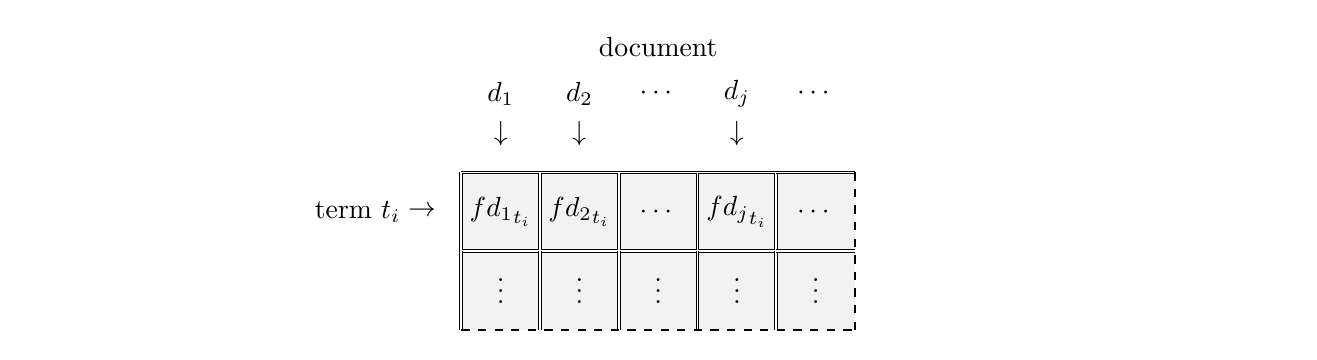
\begin{tikzpicture}
	\draw[step=1cm, opacity=0] (-5.5,0) grid (10.5,0);
	\fill[black!5!white] (0,0) rectangle (5,2);
	\draw[step=1cm, double] (0,1) grid (4,2);
	\draw[step=1cm, double] (0,0) -- (0,1);
	\draw[step=1cm, double] (1,0) -- (1,1);
	\draw[step=1cm, double] (2,0) -- (2,1);
	\draw[step=1cm, double] (3,0) -- (3,1);
	\draw[step=1cm, double] (4,0) -- (4,1);
	\draw[step=1cm, double] (4,1) -- (5,1);
	\draw[step=1cm, double] (4,2) -- (5,2);
	\draw[step=1cm, dashed] (0,0) -- (5,0);
	\draw[step=1cm, dashed] (5,0) -- (5,2);
	\node (p1) at (-0.5,1.5) {$\rightarrow$};
	\node[left=-0.15cm of p1] {term $t_i$};
	\node at (2.5,3.6) {document};
	\node at (0.5,2.5) {$\downarrow$};
	\node at (1.5,2.5) {$\downarrow$};
	\node at (3.5,2.5) {$\downarrow$};
	\node at (0.5,3) {$d_1$};
	\node at (1.5,3) {$d_2$};
	\node at (2.5,3) {$\cdots$};
	\node at (3.5,3) {$d_j$};
	\node at (4.5,3) {$\cdots$};
	\node at (0.5,1.5) {${fd_1}_{t_i}$};
	\node at (1.5,1.5) {${fd_2}_{t_i}$};
	\node at (2.5,1.5) {$\cdots$};
	\node at (3.5,1.5) {${fd_j}_{t_i}$};
	\node at (4.5,1.5) {$\cdots$};
	\node at (0.5,0.6) {$\vdots$};
	\node at (1.5,0.6) {$\vdots$};
	\node at (2.5,0.6) {$\vdots$};
	\node at (3.5,0.6) {$\vdots$};
	\node at (4.5,0.6) {$\vdots$};
\end{tikzpicture}
\caption[The term-document matrix]{The term-document matrix.\\
In a term-document matrix,
each row represents a unique term $t_i$ and
each column represents a document $d_j$.
The element ${fd_j}_{t_i}$ is the frequency of term $t_i$ in document $d_j$.}
\end{figure}

\subsection{Similarity of Words: The Word-context Matrix}
\begin{hypothesis}{Distributional Hypothesis}{}
Words that occur in similar contexts tend to have similar meanings\cite{harris1954vsmh2,firth1957vsmh2}.---If words have similar row vectors in a word-context matrix, then they tend to have similar meanings.
\end{hypothesis}
\par Researchers look into row vectors in a word-document matrix as word representations. However, documents are not the necessarily optimal contexts to understand word meanings, a word shall be known by the companies it keeps\cite{firth1957vsmh2}. Windows of words are used as contexts in Word2vec\cite{mikolov2013word2vec} and GolVe\cite{pennington2014glove}, and other linguistic information such as grammatical dependencies can also be aggregated\cite{lin1998vsmex2,pado2007vsmex2}.
\begin{figure}[t]
\small
\centering
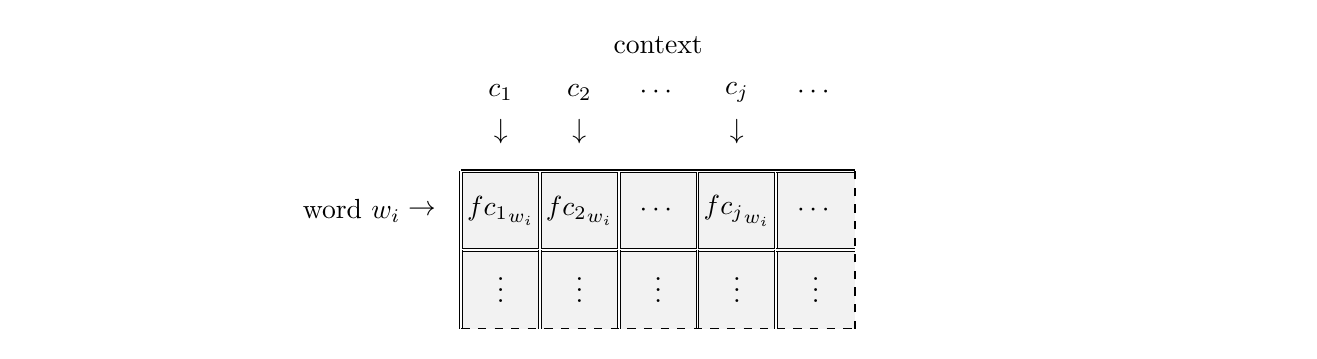
\begin{tikzpicture}
	\draw[step=1cm, opacity=0] (-5.5,0) grid (10.5,0);
	\fill[black!5!white] (0,0) rectangle (5,2);
	\draw[step=1cm, double] (0,1) grid (4,2);
	\draw[step=1cm, double] (0,0) -- (0,1);
	\draw[step=1cm, double] (1,0) -- (1,1);
	\draw[step=1cm, double] (2,0) -- (2,1);
	\draw[step=1cm, double] (3,0) -- (3,1);
	\draw[step=1cm, double] (4,0) -- (4,1);
	\draw[step=1cm, double] (4,1) -- (5,1);
	\draw[step=1cm, double] (4,2) -- (5,2);
	\draw[step=1cm, dashed] (0,0) -- (5,0);
	\draw[step=1cm, dashed] (5,0) -- (5,2);
	\node (p1) at (-0.5,1.5) {$\rightarrow$};
	\node[left=-0.15cm of p1] {word $w_i$};
	\node at (2.5,3.6) {context};
	\node at (0.5,2.5) {$\downarrow$};
	\node at (1.5,2.5) {$\downarrow$};
	\node at (3.5,2.5) {$\downarrow$};
	\node at (0.5,3) {$c_1$};
	\node at (1.5,3) {$c_2$};
	\node at (2.5,3) {$\cdots$};
	\node at (3.5,3) {$c_j$};
	\node at (4.5,3) {$\cdots$};
	\node at (0.5,1.5) {${fc_1}_{w_i}$};
	\node at (1.5,1.5) {${fc_2}_{w_i}$};
	\node at (2.5,1.5) {$\cdots$};
	\node at (3.5,1.5) {${fc_j}_{w_i}$};
	\node at (4.5,1.5) {$\cdots$};
	\node at (0.5,0.6) {$\vdots$};
	\node at (1.5,0.6) {$\vdots$};
	\node at (2.5,0.6) {$\vdots$};
	\node at (3.5,0.6) {$\vdots$};
	\node at (4.5,0.6) {$\vdots$};
\end{tikzpicture}
\caption[The word-context matrix]{The word-context matrix.\\
In a word-context matrix,
each row represents a unique word $w_i$ and
each column represents a context $c_j$.
The element ${fc_j}_{w_i}$ is the frequency of word $w_i$ in context $c_j$.}
\end{figure}

\subsection{Similarity of Relations: The Pair-pattern Matrix}
\begin{hypothesis}{Extended Distributional Hypothesis}{}
\par Patterns co-occurring with similar word-pairs tend to have similar meanings\cite{lin2001vsmh3}.---If patterns have similar column vectors in a pair-pattern matrix, then they tend to express similar semantic relations.
\end{hypothesis}
\begin{hypothesis}{Latent Relation Hypothesis}{}
\par Word-pairs co-occurring in similar patterns tend to have similar semantic relations\cite{turney2003vsmh4}.---If word pairs have similar row vectors in a pair-pattern matrix, then they tend to have similar semantic relations.
\end{hypothesis}
\par These two hypothesis are complementary concepts. The pattern ``\textsl{A eats B}" and ``\textsl{B is eaten by A}" tend to co-occur with similar word-pairs (\textsl{A}, \textsl{B}), where the extended distributional hypothesis indicates that they  may express similar semantic relations. The word-pairs (\textsl{cat}, \textsl{fish}) and (\textsl{panda}, \textsl{bamboo}) tend to co-occur with similar patter ``\textsl{A eats B}", where the latent relation hypothesis indicates that they may have similar semantic relations.
\begin{figure}[t]
\small
\centering
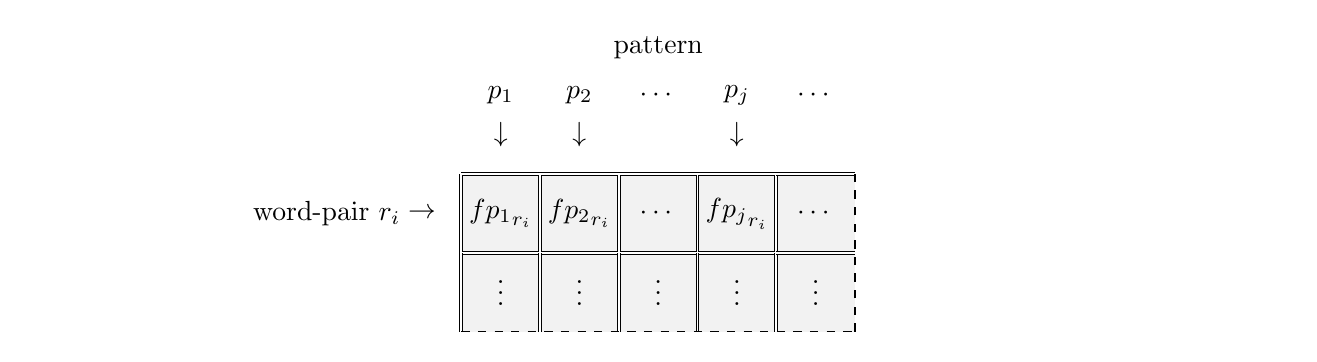
\begin{tikzpicture}
	\draw[step=1cm, opacity=0] (-5.5,0) grid (10.5,0);
	\fill[black!5!white] (0,0) rectangle (5,2);
	\draw[step=1cm, double] (0,1) grid (4,2);
	\draw[step=1cm, double] (0,0) -- (0,1);
	\draw[step=1cm, double] (1,0) -- (1,1);
	\draw[step=1cm, double] (2,0) -- (2,1);
	\draw[step=1cm, double] (3,0) -- (3,1);
	\draw[step=1cm, double] (4,0) -- (4,1);
	\draw[step=1cm, double] (4,1) -- (5,1);
	\draw[step=1cm, double] (4,2) -- (5,2);
	\draw[step=1cm, dashed] (0,0) -- (5,0);
	\draw[step=1cm, dashed] (5,0) -- (5,2);
	\node (p1) at (-0.5,1.5) {$\rightarrow$};
	\node[left=-0.15cm of p1] {word-pair $r_i$};
	\node at (2.5,3.6) {pattern};
	\node at (0.5,2.5) {$\downarrow$};
	\node at (1.5,2.5) {$\downarrow$};
	\node at (3.5,2.5) {$\downarrow$};
	\node at (0.5,3) {$p_1$};
	\node at (1.5,3) {$p_2$};
	\node at (2.5,3) {$\cdots$};
	\node at (3.5,3) {$p_j$};
	\node at (4.5,3) {$\cdots$};
	\node at (0.5,1.5) {${fp_1}_{r_i}$};
	\node at (1.5,1.5) {${fp_2}_{r_i}$};
	\node at (2.5,1.5) {$\cdots$};
	\node at (3.5,1.5) {${fp_j}_{r_i}$};
	\node at (4.5,1.5) {$\cdots$};
	\node at (0.5,0.6) {$\vdots$};
	\node at (1.5,0.6) {$\vdots$};
	\node at (2.5,0.6) {$\vdots$};
	\node at (3.5,0.6) {$\vdots$};
	\node at (4.5,0.6) {$\vdots$};
\end{tikzpicture}
\caption[The pair-pattern matrix]{The pair-pattern matrix.\\
In a pair-pattern matrix,
each row represents a unique word-pair $r_i$ and
each column represents a co-occurrence pattern $p_j$.
The element ${fp_j}_{r_i}$ is the frequency of word-pair $r_i$ in co-occurrence pattern $p_j$.}
\end{figure}

\section{Machine Learning for Text Classification}\label{sec:ml}
\par Documents are represented as vectors in a vector space model, hence any machine learning approach which works with vectors can work with vectors from a vector space model\cite{witten2016ml}. These approaches put efforts into the construction of an automatic builder of classifiers rather than a classifier\cite{sebastiani2002tc}.

\subsection{k-Nearest Neighbor Classifiers}
\par Nearest neighbor classifiers use distance such as Euclidean distance, dot product and cosine, as similarity measures to perform the classification based on the idea that instances in the same class are likely to be closer to one another than to instances in different classes.
\par For an unlabeled document, we can search the $k$-nearest neighbors among the training documents and report the majority class from these $k$ neighbors as the predicted class. The choice of $k$ typically ranges between 20 and 40 in the previous works\cite{yang1994knn,yang1999mlall,han2001knn}. Another way is searching among representative meta-documents. We summarize a meta-document for each class, then apply the same approach as mentioned above. The preprocessing phase of summarization improves the efficiency of the classifier since it significantly reduces the number of distance computations\cite{rocchio1971knn,han2000knn}.

\subsection{Naive Bayes Classifiers}
\par Generative classifiers use an implicit mixture model for generation of the underlying instances. Each component of a mixture model is essentially a generative model for a class, which provides the probability of a particular feature for that class.
\par Naive Bayes classifiers are perhaps the most common generative classifiers, they model the distribution of an instance in each class by a probabilistic distribution with independence assumptions between the distributions of features. For an unlabeled document, the component generative models are used in conjunction with the Bayes rule to compute its posterior probability of each class, and the class with the highest posterior probability is reported as the predicted class\cite{yang1999mlall,joachims1997nb,koller1997nb,lewis1998nb,mccallum1998nb,ng2002nblr}.

\subsection{Logistic Regression Classifiers}
\par Regressions are methods to discover the relationship between a dependent variable and one or more independent variables. Although these methods are designed for real values, we can treat the binary value of a class as a special case of a real value and use them in classification\cite{aggarwal2012tc}.
\par An early application is linear least squares fit (LLSF) methods. They model the binary values of classes as a linear function of features, and try to minimize the squared errors between the modeled binary values of classes and the real ones\cite{yang1994knn,yang1999mlall}. A more common application is logistic regression classifiers. Instead of modeling the binary values of classes, they model the distribution of the binary values of classes as a logistic function of a linear function, and try to maximize the probability of the real binary values\cite{ng2002nblr,zhang2003lrsvm}.

\subsection{Support Vector Machine Classifiers}
\par Support vector machines perform the classification by finding a hyperplane which best separates the different classes with the maximal margin\cite{cortes1995svm}. Besides a linear separation, tehy can construct a non-linear separation in the original space by mapping instances non-linearly to an inner product space where classes can be separated linearly. However, linear support vector machines are used most often in practice because of their simplicity\cite{aggarwal2012tc}.
\par Since the hyperplane can be determined by examining the appropriate subset of instances as support vectors around the boundaries of classes, it is effective in high dimensional spaces and suited to text classification\cite{yang1999mlall,zhang2003lrsvm,joachims1998svm,joachims1999svm,joachims2001svm}.

\subsection{Neural Network Classifiers}
\par Neural network is a collection of connected units called neurons. Each neuron receives inputs from predecessor neurons and produces outputs to successor neurons, one of each connection is associated with a weight used to compute a linear combination of inputs. An activation function or a threshold can be applied to neurons to induce non-linearity.
\par The use of multiple layers of neurons can approximate a non-linear boundary by multiple pieces of linear boundaries. The training process of such networks is more complex since the errors need to be back-propagated over different layers\cite{yang1999mlall,lam1999nn,ruiz1999nn,weigend1999nn}. However, in the case of text classification, some research observed that non-linear models do not yield significant improvement compared to linear models\cite{schutze1995nn,wiener1995nn}.
\chapter{Methodology: CopeOpi Vectors}
\section{From CopeOpi Scores to Augmented CopeOpi Scores}
\subsection{CopeOpi Scores}
\par CopeOpi scores\cite{ku2007score} are numeric sentiment scores of Chinese characters and Chinese words, which can be used to detect the sentiment polarities and measure the strength of sentiment polarities. The basic idea is that the meaning of a Chinese word is the function of its composing characters, so the sentiment of a Chinese word can also be determined from the sentiments of its composing characters.
\par They assume that Chinese characters in a Chinese positive opinion word tend to be positive, and Chinese characters in a Chinese negative opinion word tend to be negative. They adopt a Chinese sentiment dictionary, the NTU sentiment dictionary (NTUSD)\cite{ku2007ntusd}, as Chinese opinion seed words, and take the frequency of each Chinese character in these Chinese opinion seed words as clues to discover latent sentiments.
\par Once the CopeOpi scores of Chinese characters are available, the CopeOpi score of a Chinese word can be determined from the CopeOpi scores of its composing characters by applying a scoring function according to its morphological type\footnote{In linguistics, morphology is the study of the structure of words:   how words are formed, and their relationship to each other in a language.}, or simply taking the average\cite{ku2009morph}.
\input{chapters/ch3/figure/freqmat31.tex}
\begin{scheme}{CopeOpi Scores}{}
Given two corpora of labeled Chinese opinion words $\mathbb{W}_p$ and $\mathbb{W}_n$,
and the corresponding sentiment polarities $positive$ and $negative$.
\begin{itemize}
\item $\mathbb{W}_p = \{ w \where \text{$w$ is a Chinese opinion word labeled as $positive$} \}$
	\begin{itemize}
	\item the vocabulary $\mathbb{V}_p$ is a set of unique Chinese characters in $\mathbb{W}_p$
	\end{itemize}
\item $\mathbb{W}_n = \{ w \where \text{$w$ is a Chinese opinion word labeled as $negative$} \}$
	\begin{itemize}
	\item the vocabulary $\mathbb{V}_n$ is a set of unique Chinese characters in $\mathbb{W}_n$
	\end{itemize}
\end{itemize}
For each Chinese character $c_i \in \mathbb{V}_p \cup \mathbb{V}_n$,
we can compute its CopeOpi score $\mathcal{COP}_{c_i}$.
\begin{equation*}
\begin{gathered}
	\mathcal{P}_{c_i} = \dfrac{
		fp_{c_i} \divby \sum_{c \in \mathbb{V}_p} fp_c
	}{
		fp_{c_i} \divby \sum_{c \in \mathbb{V}_p} fp_c +
		fn_{c_i} \divby \sum_{c \in \mathbb{V}_n} fn_c
	}
\\[\eqlineskip]
	\mathcal{N}_{c_i} = \dfrac{
		fn_{c_i} \divby \sum_{c \in \mathbb{V}_n} fn_c
	}{
		fp_{c_i} \divby \sum_{c \in \mathbb{V}_p} fp_c +
		fn_{c_i} \divby \sum_{c \in \mathbb{V}_n} fn_c
	}
\\[\eqlineskip]
	\mathcal{COP}_{c_i} = \mathcal{P}_{c_i} - \mathcal{N}_{c_i}
\end{gathered}
\end{equation*}
where $\mathcal{P}_{c_i}$ and $\mathcal{N}_{c_i}$ are the normalized probabilities of
Chinese character $c_i$ being positive and being negative;
$fp_{c_i}$ and $fn_{c_i}$ are the frequencies of 
Chinese character $c_i$ in corpus $\mathbb{W}_p$ and in corpus $\mathbb{W}_n$;
the CopeOpi score $\mathcal{COP}_{c_i}$ of
Chinese character $c_i$ is defined as the difference of the two opposite normalized probabilities, ranged from
$+1$(being positive) to $-1$(being negative).
\tcbline
For each Chinese word $w_j=c_1c_2 \cdots c_l$, we can compute its CopeOpi score $\mathcal{COP}_{w_j}$.
\begin{equation*}
\mathcal{COP}_{w_j=c_1c_2\cdots c_l} =
\begin{cases}
	S_m(c_1c_2 \cdots c_l)
	& \text{if the morphological type of $w_j$ is $m$}
\\
	\dfrac{1}{l} \sum_{k=1}^l \mathcal{COP}_{c_k}
	& \text{otherwise}
\end{cases}
\end{equation*}
where $S_m$ is the scoring function of morphological type $m$.
\end{scheme}
One application of CopeOpi scores is augmented NTU sentiment dictionary (ANTUSD)\cite{wang2006antusd}, a collection of sentiment statistics of Chinese words in several sentiment annotation works. For each Chinese  word in the dictionary, the number of positive annotations, neutral annotations, negative annotations, non-opinionated annotations and not-a-word annotations are recorded, and the CopeOpi score is also provided.
\subsection{Augmented CopeOpi Scores}
\par The structure of the frequency matrix of CopeOpi scores relates to its potential applications. In the frequency matrix of CopeOpi scores, the basic units are Chinese characters and the contexts are corpora of labeled Chinese opinion words, so CopeOpi scores find their applications in Chinese sentiment analysis.
\par However, since the core of CopeOpi scores is a bag-of-units method which is generally adopted in nature language processing, we think it is possible to augment their usefulness and widen their range of applications.
\par Here we propose a new computation scheme for augmented CopeOpi scores. We transform CopeOpi scores from sentiment scores to class-tendency scores by mapping the sentiment polarities in sentiment analysis, i.e., positive or negative, to the set membership in binary classification, i.e., being in a class or not. We extend the premises and assume that words in documents of some classes tend to be in those classes. We modify the structure of the frequency matrix and
\begin{itemize}
\item change the basic units from Chinese characters to words.
\item change the contexts from corpora of Chinese opinion words to corpora of binary annotated documents.
\end{itemize}
\begin{figure}[t]
\small
\centering
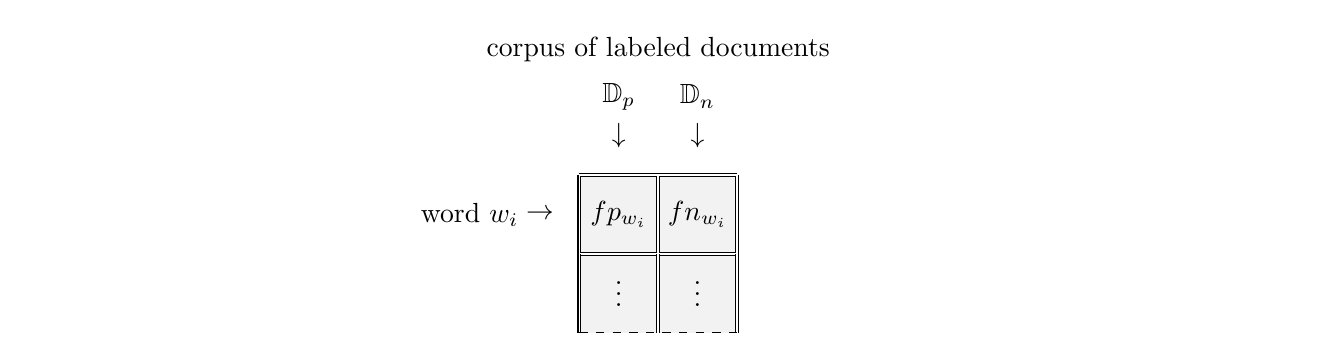
\begin{tikzpicture}
	\draw[step=1cm, opacity=0] (-7,0) grid (9,0);
	\fill[black!5!white] (0,0) rectangle (2,2);
	\draw[step=1cm, double] (0,1) grid (2,2);
	\draw[step=1cm, double] (0,0) -- (0,1);
	\draw[step=1cm, double] (1,0) -- (1,1);
	\draw[step=1cm, double] (2,0) -- (2,1);
	\draw[step=1cm, dashed] (0,0) -- (2,0);
	\node (p1) at (-0.5,1.5) {$\rightarrow$};
	\node[left=-0.15cm of p1] {word $w_i$};
	\node at (1.0,3.6) {corpus of labeled documents};
	\node at (0.5,2.5) {$\downarrow$};
	\node at (1.5,2.5) {$\downarrow$};
	\node at (0.5,3) {$\mathbb{D}_p$};
	\node at (1.5,3) {$\mathbb{D}_n$};
	\node at (0.5,1.5) {$fp_{w_i}$};
	\node at (1.5,1.5) {$fn_{w_i}$};
	\node at (0.5,0.6) {$\vdots$};
	\node at (1.5,0.6) {$\vdots$};
\end{tikzpicture}
\caption[The frequency matrix of augmented CopeOpi scores]{The frequency matrix of augmented CopeOpi scores.\\
In the frequency matrix of augmented CopeOpi scores,
each row represents a unique word $w_i$ and
the two columns represent two corpora of labeled documents $\mathbb{D}_p$ and $\mathbb{D}_n$.
The elements $fp_{w_i}$ and $fn_{w_i}$ are the frequencies of word $w_i$ 
in corpus $\mathbb{D}_p$ and in corpus $\mathbb{D}_n$.}
\end{figure}
\begin{scheme}{Augmented CopeOpi Scores}{}
Given two corpora of labeled documents $\mathbb{D}_p$ and $\mathbb{D}_n$,
and the corresponding classes $p$ and $not\text{-}p$.
\begin{itemize}
\item $\mathbb{D}_p = \{ \langle d,c \rangle \where \text{$d$ is a document labeled as class $c=p$} \}$
	\begin{itemize}
	\item the vocabulary $\mathbb{V}_p$ is a set of unique words in $\mathbb{D}_p$
	\end{itemize}
\item $\mathbb{D}_n = \{ \langle d,c \rangle \where \text{$d$ is a document labeled as class $c=not\text{-}p$} \}$
	\begin{itemize}
	\item the vocabulary $\mathbb{V}_n$ is a set of unique words in $\mathbb{D}_n$
	\end{itemize}
\end{itemize}
For each word $w_i \in \mathbb{V}_p \cup \mathbb{V}_n$,
we can compute its CopeOpi score $\mathcal{COP}_{w_i}$.
\begin{equation*}
\begin{gathered}
	\mathcal{P}_{w_i} = \dfrac{
		fp_{w_i} \divby \sum_{w \in \mathbb{V}_p} fp_w
	}{
		fp_{w_i} \divby \sum_{w \in \mathbb{V}_p} fp_w +
		fn_{w_i} \divby \sum_{w \in \mathbb{V}_n} fn_w
	}
\\[\eqlineskip]
	\mathcal{N}_{w_i} = \dfrac{
		fn_{w_i} \divby \sum_{w \in \mathbb{V}_n} fn_w
	}{
		fp_{w_i} \divby \sum_{w \in \mathbb{V}_p} fp_w +
		fn_{w_i} \divby \sum_{w \in \mathbb{V}_n} fn_w
	}
\\[\eqlineskip]
	\mathcal{COP}_{w_i} = \mathcal{P}_{w_i} - \mathcal{N}_{w_i}
\end{gathered}
\end{equation*}
where $\mathcal{P}_{w_i}$ and $\mathcal{N}_{w_i}$ are the normalized probabilities of
word $w_i$ being in class $p$ and being in class $not\text{-}p$;
$fp_{w_i}$ and $fn_{w_i}$ are the frequencies of 
word $w_i$ in corpus $\mathbb{D}_p$ and in corpus $\mathbb{D}_n$;
the CopeOpi score $\mathcal{COP}_{w_i}$ of
word $w_i$ is defined as the difference of the two opposite normalized probabilities, ranged from
$+1$(being in class $p$) to $-1$(being in class $not\text{-}p$).
\end{scheme}
\partopic{Confidence in Augmented CopeOpi Scores}
\par According to Zipf's law, given some corpora of natural language, the frequency of a word is inversely proportional to its rank in the frequency table\cite{manning1999nlp}. The most frequent word occurs approximately twice as often as the second one, three times as often as the third one, etc. There are a few words that are very common and a lot of words that are very rare. Considering the later cases, we shall have less confidence in the augmented CopeOpi scores of rare words due to the lack of sufficient statistics, and besides, they are easily biased and overestimated since the occurrences of a rare word might be all in one class and absent in the other.
\par To reduce the effects of imprecise augmented CopeOpi scores of rare words, we can impose confidence values to penalize these values. We regard words whose maximal class frequency less than the average class frequency of all words as rare words, and smooth their augmented CopeOpi scores by multiplying their confidence values which is defined as a logistic function\footnote{The mentioned scheme of confidence values is merely the one we use in our experiments but not a standard scheme. You can design one for your applications.}.
\begin{equation*}
\begin{gathered}
	fc^{\max}_{w_i} = \max({fc_1}_{w_i},{fc_2}_{w_i},\dots,{fc_n}_{w_i})
\\[\eqlineskip]
	fc_{\avg} = \dfrac {
		\sum_{j=1}^m \sum_{k=1}^n {fc_k}_{w_j}
	}{
		m \times n
	}
\\[\eqlineskip]
	\mathcal{CF}_{w_i} =
	\begin{cases}
		1
		&\text{if $fc^{\max}_{w_i} \geq fc_{\avg}$}
	\\
		\dfrac{1}{1 + 3 \exp(-4(\frac{fc^{\max}_{w_i}}{fc_{\avg}}))}
		&\text{otherwise}
	\end{cases}
\\[\eqlineskip]
	\mathcal{CF}\text{-}\mathcal{COP}_{w_i} = \mathcal{CF}_{w_i} \times \mathcal{COP}_{w_i}
\end{gathered}
\end{equation*}
where ${fc_k}_{w_i}$ is the frequency of word $w_i$ in class $k$;
$fc^{\max}_{w_i}$ and $fc_{\avg}$ are the maximal class frequency of word $w_i$ and the average class frequency of all words;
$n$ and $m$ are the number of classes and the number unique words in corpora;
the confidence value $\mathcal{CF}_{w_i}$ of word $w_i$ is defined as a piece-wise function which behaves differently based on the maximal class frequency $fc^{\max}_{w_i}$ of word $w_i$.
\begin{figure}[t]
\begin{minipage}{0.5\textwidth}
	\centering
	\includegraphics[height=6cm]{chapters/ch3/figure/conf.png}
	\caption{The logistic function of $\mathcal{CF}$}
\end{minipage}
\begin{minipage}{0.5\textwidth}
	\centering
	\includegraphics[height=6cm]{chapters/ch3/figure/conf_ex.png}
	\caption{Distributions of $\mathcal{COP}$ and $\mathcal{CF}\text{-}\mathcal{COP}$}
\end{minipage}
\end{figure}

\section{From Augmented CopeOpi Scores to CopeOpi Vectors}
\subsection{CopeOpi Vectors}
\par CopeOpi scores now become augmented CopeOpi scores, class-tendency scores which can be used in languages other than Chinese since we change the basic units from Chinese characters to words, and be applied to binary text classification other than sentiment analysis since we change the contexts from corpora of Chinese opinion words to corpora of binary annotated documents.
\par However, there are many text classification problems with more than two classes. Augmented CopeOpi scores can not help solve them due to the fact that they are scalars and can represent at most two oppositions by being positive or being negative.
\par Here we find a way to make augmented CopeOpi scores applicable to multiclass text classification. We expand augmented CopeOpi scores to CopeOpi vectors by utilizing divide-and-conquer techniques for multiclass classification. We decompose a multiclass text classification problem into multiple binary text classification subproblems, and compute an augmented CopeOpi score for each subproblem as a component of CopeOpi vectors. Several strategies have been proposed for such a decomposition\cite{aly2005multiclass}.
\begin{figure}[t]
\small
\centering
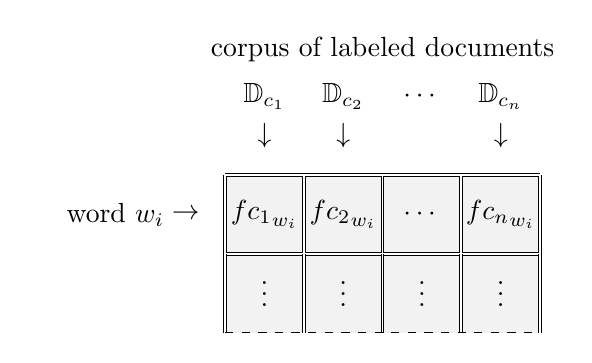
\begin{tikzpicture}
	\draw[step=1cm, opacity=0] (-2.5,0) grid (4,0);
	\fill[black!5!white] (0,0) rectangle (4,2);
	\draw[step=1cm, double] (0,1) grid (4,2);
	\draw[step=1cm, double] (0,0) -- (0,1);
	\draw[step=1cm, double] (1,0) -- (1,1);
	\draw[step=1cm, double] (2,0) -- (2,1);
	\draw[step=1cm, double] (3,0) -- (3,1);
	\draw[step=1cm, double] (4,0) -- (4,1);
	\draw[step=1cm, dashed] (0,0) -- (4,0);
	\node (p1) at (-0.5,1.5) {$\rightarrow$};
	\node[left=-0.15cm of p1] {word $w_i$};
	\node at (2.0,3.6) {corpus of labeled documents};
	\node at (0.5,2.5) {$\downarrow$};
	\node at (1.5,2.5) {$\downarrow$};
	\node at (3.5,2.5) {$\downarrow$};
	\node at (0.5,3) {$\mathbb{D}_{c_1}$};
	\node at (1.5,3) {$\mathbb{D}_{c_2}$};
	\node at (2.5,3) {$\cdots$};
	\node at (3.5,3) {$\mathbb{D}_{c_n}$};
	\node at (0.5,1.5) {${fc_1}_{w_i}$};
	\node at (1.5,1.5) {${fc_2}_{w_i}$};
	\node at (2.5,1.5) {$\cdots$};
	\node at (3.5,1.5) {${fc_n}_{w_i}$};
	\node at (0.5,0.6) {$\vdots$};
	\node at (1.5,0.6) {$\vdots$};
	\node at (2.5,0.6) {$\vdots$};
	\node at (3.5,0.6) {$\vdots$};
\end{tikzpicture}
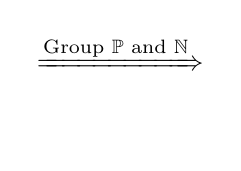
\begin{tikzpicture}
	\draw[step=1cm, opacity=0] (0,0) grid (1,0);
	\node at (0,1) {$\xRightarrow{\text{Group $\mathbb{P}$ and $\mathbb{N}$}}$};
\end{tikzpicture}
\hspace{-1cm}
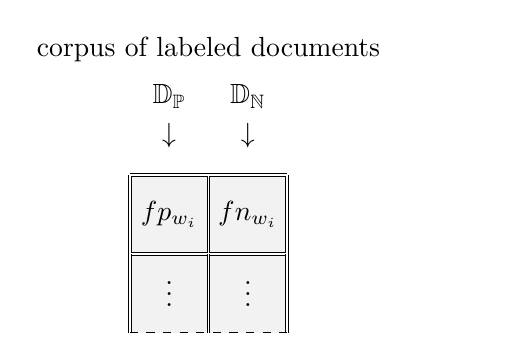
\begin{tikzpicture}
	\draw[step=1cm, opacity=0] (0,0) grid (4.5,0);
	\fill[black!5!white] (0,0) rectangle (2,2);
	\draw[step=1cm, double] (0,1) grid (2,2);
	\draw[step=1cm, double] (0,0) -- (0,1);
	\draw[step=1cm, double] (1,0) -- (1,1);
	\draw[step=1cm, double] (2,0) -- (2,1);
	\draw[step=1cm, dashed] (0,0) -- (2,0);
	%\node (p1) at (-0.5,1.5) {$\rightarrow$};
	%\node[left=-0.15cm of p1] {word $w_i$};
	\node at (1.0,3.6) {corpus of labeled documents};
	\node at (0.5,2.5) {$\downarrow$};
	\node at (1.5,2.5) {$\downarrow$};
	\node at (0.5,3) {$\mathbb{D}_\mathbb{P}$};
	\node at (1.5,3) {$\mathbb{D}_\mathbb{N}$};
	\node at (0.5,1.5) {$fp_{w_i}$};
	\node at (1.5,1.5) {$fn_{w_i}$};
	\node at (0.5,0.6) {$\vdots$};
	\node at (1.5,0.6) {$\vdots$};
\end{tikzpicture}
\caption[The frequency matrix of CopeOpi vectors]{The frequency matrix of CopeOpi vectors.\\
In the frequency matrix of CopeOpi vectors,
each row represents a unique word $w_i$ and
the $n$ columns represent $n$ corpora of labeled documents $\mathbb{D}_{c_1},\mathbb{D}_{c_2},\dots,\mathbb{D}_{c_n}$.
The element ${fc_j}_{w_i}$ is the frequency of word $w_i$
in corpus $\mathbb{D}_{c_j}$.
After $\mathbb{P}$ and $\mathbb{N}$ are grouped,
the two columns represent two corpora of labeled documents $\mathbb{D}_\mathbb{P}$ and $\mathbb{D}_\mathbb{N}$.
The elements $fp_{w_i}$ and $fn_{w_i}$ are the frequencies of word $w_i$ 
in corpus $\mathbb{D}_\mathbb{P}$ and in corpus $\mathbb{D}_\mathbb{N}$.}
\end{figure}
~\newline
~\newline
\clearpage
\partopic{One-versus-Rest\footnote{Also known as one-versus-all (OVA), one-against-rest (OAR), one-against-all (OAA).} Strategy (OVR)}
\par In an $n$-class text classification problem, we require $n$ augmented CopeOpi scores,
where each augmented CopeOpi score is computed to discriminate between one of the classes and the rest of the classes.
\begin{scheme}{CopeOpi Vectors (One-versus-Rest)}{}
Given $n$ corpora of labeled documents $\mathbb{D} = \{ \mathbb{D}_{c_1},\mathbb{D}_{c_2},\dots,\mathbb{D}_{c_n} \}$,
and the corresponding classes $\mathbb{C} = \{ c_1,c_2,\dots,c_n \}$.
\begin{itemize}
\item $\mathbb{D}_{c_i} = \{ \langle d,c \rangle \where \text{$d$ is a document labeled as class $c=c_i$} \}$
	\begin{itemize}
	\item the vocabulary $\mathbb{V}_{c_i}$ is a set of unique words in $\mathbb{D}_{c_i}$
	\end{itemize}
\end{itemize}
For each word $w_i \in \cup_{c \in \mathbb{C}} \mathbb{V}_{c}$,
we can compute its CopeOpi vector $\overrightarrow{\mathcal{COP}}_{w_i}$ by one-versus-rest strategy.
\tcbline
For each class $c_j \in \mathbb{C}$, we can construct two opposite sets,
\begin{itemize}
\item the positive set $\mathbb{P}^{c_j}_{w_i} = \{ c_j \}$
	\begin{itemize}
	\item the positive corpus ${\mathbb{D}_\mathbb{P}}^{c_j}_{w_i} = \{ \mathbb{D}_{c_j} \}$
	\item the positive vocabulary ${\mathbb{V}_\mathbb{P}}^{c_j}_{w_i} = \mathbb{V}_{c_j}$
	\end{itemize}
\item the negative set $\mathbb{N}^{c_j}_{w_i} = \mathbb{C} \setminus \{ c_j \}$
	\begin{itemize}
	\item the negative corpus ${\mathbb{D}_\mathbb{N}}^{c_j}_{w_i} = \mathbb{D} \setminus \{ \mathbb{D}_{c_j} \}$
	\item the negative vocabulary ${\mathbb{V}_\mathbb{N}}^{c_j}_{w_i} = \cup_{c \in \mathbb{N}^{c_j}_{w_i}} \mathbb{V}_{c}$
	\end{itemize}
\end{itemize}
and compute the augmented CopeOpi score $\mathcal{COP}^{c_j}_{w_i}$
of word $w_i$ with respect to class $c_j$ based on these two opposite sets.
\begin{equation*}
\begin{gathered}
	\mathcal{P}^{c_j}_{w_i} = \dfrac{
		fp^{c_j}_{w_i} \divby \sum_{w \in {\mathbb{V}_\mathbb{P}}^{c_j}_{w_i}} fp^{c_j}_w
	}{
		fp^{c_j}_{w_i} \divby \sum_{w \in {\mathbb{V}_\mathbb{P}}^{c_j}_{w_i}} fp^{c_j}_w +
		fn^{c_j}_{w_i} \divby \sum_{w \in {\mathbb{V}_\mathbb{N}}^{c_j}_{w_i}} fn^{c_j}_w
	}
\\[\eqlineskip]
	\mathcal{N}^{c_j}_{w_i} = \dfrac{
		fn^{c_j}_{w_i} \divby \sum_{w \in {\mathbb{V}_\mathbb{N}}^{c_j}_{w_i}} fn^{c_j}_w
	}{
		fp^{c_j}_{w_i} \divby \sum_{w \in {\mathbb{V}_\mathbb{P}}^{c_j}_{w_i}} fp^{c_j}_w +
		fn^{c_j}_{w_i} \divby \sum_{w \in {\mathbb{V}_\mathbb{N}}^{c_j}_{w_i}} fn^{c_j}_w
	}
\\[\eqlineskip]
	\mathcal{COP}^{c_j}_{w_i} = \mathcal{P}^{c_j}_{w_i} - \mathcal{N}^{c_j}_{w_i}
\end{gathered}
\end{equation*}
where $\mathcal{P}^{c_j}_{w_i}$ and $\mathcal{N}^{c_j}_{w_i}$ are the normalized probabilities of
word $w_i$ being in class $\mathbb{P}^{c_j}_{w_i}$ and being in class $\mathbb{N}^{c_j}_{w_i}$;
$fp^{c_j}_{w_i}$ and $fn^{c_j}_{w_i}$ are the frequencies of 
word $w_i$ in corpus ${\mathbb{D}_\mathbb{P}}^{c_j}_{w_i}$ and in corpus ${\mathbb{D}_\mathbb{N}}^{c_j}_{w_i}$;
the CopeOpi score $\mathcal{COP}^{c_j}_{w_i}$ of
word $w_i$ with respect to class $c_j$ is defined as the difference of the two opposite normalized probabilities, ranged from
$+1$(being in class $\mathbb{P}^{c_j}_{w_i}$) to $-1$(being in class $\mathbb{N}^{c_j}_{w_i}$).
\vspace{1.3\baselineskip}
\tcbline
The CopeOpi vector $\overrightarrow{\mathcal{COP}}_{w_i}$ of word $w_i$ is composed of these $n$ augmented CopeOpi scores.
~\newline
\begin{equation*}
\overrightarrow{\mathcal{COP}}_{w_i} = (\mathcal{COP}^{c_1}_{w_i},\mathcal{COP}^{c_2}_{w_i},\dots,\mathcal{COP}^{c_n}_{w_i})
\end{equation*}
\end{scheme}
\partopic{One-versus-One\footnote{Also known as one-against-one (OAO).} Strategy (OVO)}
\par In an $n$-class text classification problem, we require $\frac{1}{2}n(n-1)$ augmented CopeOpi scores,
where each augmented CopeOpi score is computed to discriminate between a pair of classes.
\begin{scheme}{CopeOpi Vectors (One-versus-One)}{}
Given $n$ corpora of labeled documents $\mathbb{D} = \{ \mathbb{D}_{c_1},\mathbb{D}_{c_2},\dots,\mathbb{D}_{c_n} \}$,
and the corresponding classes $\mathbb{C} = \{ c_1,c_2,\dots,c_n \}$.
\begin{itemize}
\item $\mathbb{D}_{c_i} = \{ \langle d,c \rangle \where \text{$d$ is a document labeled as class $c=c_i$} \}$
	\begin{itemize}
	\item the vocabulary $\mathbb{V}_{c_i}$ is a set of unique words in $\mathbb{D}_{c_i}$
	\end{itemize}
\end{itemize}
For each word $w_i \in \cup_{c \in \mathbb{C}} \mathbb{V}_{c}$,
we can compute its CopeOpi vector $\overrightarrow{\mathcal{COP}}_{w_i}$ by one-versus-one strategy.
\tcbline
For each class-pair $c_j,c_k \in \mathbb{C}$, $1 \leq j < k \leq n$, we can construct two opposite sets,
\begin{itemize}
\item the positive set $\mathbb{P}^{c_j,c_k}_{w_i} = \{ c_j \}$
	\begin{itemize}
	\item the positive corpus ${\mathbb{D}_\mathbb{P}}^{c_j,c_k}_{w_i} = \{ \mathbb{D}_{c_j} \}$
	\item the positive vocabulary ${\mathbb{V}_\mathbb{P}}^{c_j,c_k}_{w_i} = \mathbb{V}_{c_j}$
	\end{itemize}
\item the negative set $\mathbb{N}^{c_j,c_k}_{w_i} = \{ c_k \}$
	\begin{itemize}
	\item the negative corpus ${\mathbb{D}_\mathbb{N}}^{c_j,c_k}_{w_i} = \{ \mathbb{D}_{c_k} \}$
	\item the negative vocabulary ${\mathbb{V}_\mathbb{N}}^{c_j,c_k}_{w_i} = \mathbb{V}_{c_k}$
	\end{itemize}
\end{itemize}
and compute the augmented CopeOpi score $\mathcal{COP}^{c_j,c_k}_{w_i}$
of word $w_i$ with respect to class-pair $c_j,c_k$ based on these two opposite sets.

\begin{equation*}
\begin{gathered}
	\mathcal{P}^{c_j,c_k}_{w_i} = \dfrac{
		fp^{c_j,c_k}_{w_i} \divby \sum_{w \in {\mathbb{V}_\mathbb{P}}^{c_j,c_k}_{w_i}} fp^{c_j,c_k}_w
	}{
		fp^{c_j,c_k}_{w_i} \divby \sum_{w \in {\mathbb{V}_\mathbb{P}}^{c_j,c_k}_{w_i}} fp^{c_j,c_k}_w +
		fn^{c_j,c_k}_{w_i} \divby \sum_{w \in {\mathbb{V}_\mathbb{N}}^{c_j,c_k}_{w_i}} fn^{c_j,c_k}_w
	}
\\[\eqlineskip]
	\mathcal{N}^{c_j,c_k}_{w_i} = \dfrac{
		fn^{c_j,c_k}_{w_i} \divby \sum_{w \in {\mathbb{V}_\mathbb{N}}^{c_j,c_k}_{w_i}} fn^{c_j,c_k}_w
	}{
		fp^{c_j,c_k}_{w_i} \divby \sum_{w \in {\mathbb{V}_\mathbb{P}}^{c_j,c_k}_{w_i}} fp^{c_j,c_k}_w +
		fn^{c_j,c_k}_{w_i} \divby \sum_{w \in {\mathbb{V}_\mathbb{N}}^{c_j,c_k}_{w_i}} fn^{c_j,c_k}_w
	}
\\[\eqlineskip]
	\mathcal{COP}^{c_j,c_k}_{w_i} = \mathcal{P}^{c_j,c_k}_{w_i} - \mathcal{N}^{c_j,c_k}_{w_i}
\end{gathered}
\end{equation*}
where $\mathcal{P}^{c_j,c_k}_{w_i}$ and $\mathcal{N}^{c_j,c_k}_{w_i}$ are the normalized probabilities of
word $w_i$ being in class $\mathbb{P}^{c_j,c_k}_{w_i}$ and being in class $\mathbb{N}^{c_j,c_k}_{w_i}$;
$fp^{c_j,c_k}_{w_i}$ and $fn^{c_j,c_k}_{w_i}$ are the frequencies of 
word $w_i$ in corpus ${\mathbb{D}_\mathbb{P}}^{c_j,c_k}_{w_i}$ and in corpus ${\mathbb{D}_\mathbb{N}}^{c_j,c_k}_{w_i}$;
the CopeOpi score $\mathcal{COP}^{c_j,c_k}_{w_i}$ of
word $w_i$ with respect to class-pair $c_j,c_k$ is defined as the difference of the two opposite normalized probabilities, ranged from
$+1$(being in class $\mathbb{P}^{c_j,c_k}_{w_i}$) to $-1$(being in class $\mathbb{N}^{c_j,c_k}_{w_i}$).
\tcbline
The CopeOpi vector $\overrightarrow{\mathcal{COP}}_{w_i}$ of word $w_i$ is composed of these $\frac{1}{2}n(n-1)$ augmented CopeOpi scores.
\begin{equation*}
\overrightarrow{\mathcal{COP}}_{w_i} = (\mathcal{COP}^{c_1,c_2}_{w_i},\mathcal{COP}^{c_1,c_3}_{w_i},\dots,\mathcal{COP}^{c_{n-1},c_n}_{w_i})
\end{equation*}
\end{scheme}

\clearpage
\subsection{Customized CopeOpi Vectors}\label{sec:customized}
\par One-versus-rest strategy and one-versus-one strategy guide the basic way to construct CopeOpi vectors which can be applied to multiclass text classification.
\par However, in general, any subset of classes can be grouped as a positive set or a negative set. CopeOpi vectors can be customized based on different choices of subset-pairs.
~\newline
~\newline
\partopic{Subset-versus-Subset Strategy (SVS)}
\par In an $n$-class text classification problem, we can have at most $(2^n-1)^2$ augmented CopeOpi scores\footnote{We only eliminate the empty set cases, but not all subset-pairs can produce a discriminative augmented CopeOpi score.},
where each augmented CopeOpi score is computed to discriminate between a pair of subsets of classes.
\begin{scheme}{CopeOpi Vectors (Subset-versus-Subset)}{}
Given $n$ corpora of labeled documents $\mathbb{D} = \{ \mathbb{D}_{c_1},\mathbb{D}_{c_2},\dots,\mathbb{D}_{c_n} \}$,
and the corresponding classes $\mathbb{C} = \{ c_1,c_2,\dots,c_n \}$.
\begin{itemize}
\item $\mathbb{D}_{c_i} = \{ \langle d,c \rangle \where \text{$d$ is a document labeled as class $c=c_i$} \}$
	\begin{itemize}
	\item the vocabulary $\mathbb{V}_{c_i}$ is a set of unique words in $\mathbb{D}_{c_i}$
	\end{itemize}
\end{itemize}
For each word $w_i \in \cup_{c \in \mathbb{C}} \mathbb{V}_{c}$,
we can compute its CopeOpi vector $\overrightarrow{\mathcal{COP}}_{w_i}$ by subset-versus-subset strategy.
\tcbline
For any subset-pair $\mathbb{J},\mathbb{K} \subseteq \mathbb{C}$ where $\mathbb{J},\mathbb{K} \neq \varnothing$, can construct two opposite sets,
\begin{itemize}
\item the positive set $\mathbb{P}^{\mathbb{J},\mathbb{K}}_{w_i} = \mathbb{J}$
	\begin{itemize}
	\item the positive corpus ${\mathbb{D}_\mathbb{P}}^{\mathbb{J},\mathbb{K}}_{w_i} = \{ \mathbb{D}_{c} \where c \in \mathbb{J} \}$
	\item the positive vocabulary ${\mathbb{V}_\mathbb{P}}^{\mathbb{J},\mathbb{K}}_{w_i} = \cup_{c \in \mathbb{J}} \mathbb{V}_{c}$
	\end{itemize}
\item the positive set $\mathbb{N}^{\mathbb{J},\mathbb{K}}_{w_i} = \mathbb{K}$
	\begin{itemize}
	\item the positive corpus ${\mathbb{D}_\mathbb{N}}^{\mathbb{J},\mathbb{K}}_{w_i} = \{ \mathbb{D}_{c} \where c \in \mathbb{K} \}$
	\item the positive vocabulary ${\mathbb{V}_\mathbb{N}}^{\mathbb{J},\mathbb{K}}_{w_i} = \cup_{c \in \mathbb{K}} \mathbb{V}_{c}$
	\end{itemize}
\end{itemize}
and compute the augmented CopeOpi score $\mathcal{COP}^{\mathbb{J},\mathbb{K}}_{w_i}$
of word $w_i$ with respect to subset-pair $\mathbb{J},\mathbb{K}$ based on these two opposite sets.
\begin{equation*}
\begin{gathered}
	\mathcal{P}^{\mathbb{J},\mathbb{K}}_{w_i} = \dfrac{
		fp^{\mathbb{J},\mathbb{K}}_{w_i} \divby \sum_{w \in {\mathbb{V}_\mathbb{P}}^{\mathbb{J},\mathbb{K}}_{w_i}} fp^{\mathbb{J},\mathbb{K}}_w
	}{
		fp^{\mathbb{J},\mathbb{K}}_{w_i} \divby \sum_{w \in {\mathbb{V}_\mathbb{P}}^{\mathbb{J},\mathbb{K}}_{w_i}} fp^{\mathbb{J},\mathbb{K}}_w +
		fn^{\mathbb{J},\mathbb{K}}_{w_i} \divby \sum_{w \in {\mathbb{V}_\mathbb{N}}^{\mathbb{J},\mathbb{K}}_{w_i}} fn^{\mathbb{J},\mathbb{K}}_w
	}
\\[\eqlineskip]
	\mathcal{N}^{\mathbb{J},\mathbb{K}}_{w_i} = \dfrac{
		fn^{\mathbb{J},\mathbb{K}}_{w_i} \divby \sum_{w \in {\mathbb{V}_\mathbb{N}}^{\mathbb{J},\mathbb{K}}_{w_i}} fn^{\mathbb{J},\mathbb{K}}_w
	}{
		fp^{\mathbb{J},\mathbb{K}}_{w_i} \divby \sum_{w \in {\mathbb{V}_\mathbb{P}}^{\mathbb{J},\mathbb{K}}_{w_i}} fp^{\mathbb{J},\mathbb{K}}_w +
		fn^{\mathbb{J},\mathbb{K}}_{w_i} \divby \sum_{w \in {\mathbb{V}_\mathbb{N}}^{\mathbb{J},\mathbb{K}}_{w_i}} fn^{\mathbb{J},\mathbb{K}}_w
	}
\\[\eqlineskip]
	\mathcal{COP}^{\mathbb{J},\mathbb{K}}_{w_i} = \mathcal{P}^{\mathbb{J},\mathbb{K}}_{w_i} - \mathcal{N}^{\mathbb{J},\mathbb{K}}_{w_i}
\end{gathered}
\end{equation*}
where $\mathcal{P}^{\mathbb{J},\mathbb{K}}_{w_i}$ and $\mathcal{N}^{\mathbb{J},\mathbb{K}}_{w_i}$ are the normalized probabilities of
word $w_i$ being in class $\mathbb{P}^{\mathbb{J},\mathbb{K}}_{w_i}$ and being in class $\mathbb{N}^{\mathbb{J},\mathbb{K}}_{w_i}$;
$fp^{\mathbb{J},\mathbb{K}}_{w_i}$ and $fn^{\mathbb{J},\mathbb{K}}_{w_i}$ are the frequencies of 
word $w_i$ in corpus ${\mathbb{D}_\mathbb{P}}^{\mathbb{J},\mathbb{K}}_{w_i}$ and in corpus ${\mathbb{D}_\mathbb{N}}^{\mathbb{J},\mathbb{K}}_{w_i}$;
the CopeOpi score $\mathcal{COP}^{\mathbb{J},\mathbb{K}}_{w_i}$ of
word $w_i$ with respect to subset-pair $\mathbb{J},\mathbb{K}$ is defined as the difference of the two opposite normalized probabilities, ranged from
$+1$(being in class $\mathbb{P}^{\mathbb{J},\mathbb{K}}_{w_i}$) to $-1$(being in class $\mathbb{N}^{\mathbb{J},\mathbb{K}}_{w_i}$).
\tcbline
The CopeOpi vector $\overrightarrow{\mathcal{COP}}_{w_i}$ of word $w_i$ is composed of these at most $(2^n-1)^2$ augmented CopeOpi scores.
\begin{equation*}
\overrightarrow{\mathcal{COP}}_{w_i} = (\mathcal{COP}^{\mathbb{J}_1,\mathbb{K}_1}_{w_i},\mathcal{COP}^{\mathbb{J}_2,\mathbb{K}_2}_{w_i},\dots)
\end{equation*}
\end{scheme}
\chapter{Experiments and Results}
\par To verify the functionality of CopeOpi vectors, we make comparisons with several commonly-used features for text classificaiton, and examine these features on different types of machine learning algorithms to solve text classification problems, including sentiment analysis and topic categorization, in both English and Chinese.
\section{Flowchart and Settings}
\par Figure~\ref{fig:flowchart} shows the flowchart of our experiments, detailed settings are described in the following sections.
\begin{figure}[h]
	\centering
	\includegraphics[scale=0.42]{chapters/ch4/figure/flowchart.png}
	\caption{The flowchart of experiments}
	\label{fig:flowchart}
\end{figure}
\par Table~\ref{tab:flow_opensrc} lists the open sources used in our experiments. They provide high quality implementation and ensure the reliability of experiment results.
\begin{table}[h]
\footnotesize
\centering
\caption{The open sources used in experiments}
\label{tab:flow_opensrc}
\begin{tabular}{|l|l|c|}
	\hline
	\multicolumn{1}{|c|}{Open Source}                                            & \multicolumn{1}{c|}{Functions}     & Reference                   \\ \hline
	\texttt{scikit-learn}\tablefootnote{http://scikit-learn.org}                 & Machine learning toolbox           & \cite{sklearn}              \\ \hline
	\texttt{gensim}\tablefootnote{http://radimrehurek.com/gensim}                & Nature language processing toolbox & \cite{gensim}               \\ \hline
	Stanford GloVe Project\tablefootnote{http://nlp.stanford.edu/projects/glove} & GloVe implementation                & \cite{pennington2014glove}  \\ \hline
	\texttt{jieba}\tablefootnote{http://github.com/fxsjy/jieba}                  & Chinese word segmenter             & \cite{jieba}                \\ \hline
\end{tabular}
\end{table}

\subsection{Sampling}
\par In most operational machine learning settings, once a classifier has been constructed, it is desirable to evaluate its performance. In this case, prior to classifier construction, the initial dataset is split into two parts\cite{sebastiani2002tc,ripley2007ml}:
\begin{itemize}
\item training set: a set of labeled instances used to construct a classifier, to fit the parameters of a machine learning algorithm.
	\begin{itemize}
	\item validation set: a set of labeled instances used to tune the hyperparameters of a machine learning algorithm.
	\end{itemize}
\item testing set: a set of labeled instances used to evaluate a classifier, to assess the performance of a fully-specified classifier.
\end{itemize}
~\newline
\partopic{Experiment Settings} are described in the sections of experiments.

\subsection{Preprocessing}
\par It is useful to apply some linguistic processing to raw texts before performing an analysis on them. Things to consider include:
\begin{itemize}
\item text cleaning: stripping unwanted tags, punctuation, numeric, etc.
\item tokenization: deciding what constitutes a unit and how to extract units.
\item normalization: converting superficially-different units to the same form.
\item stopword removal: removing frequent words which do not carry much meaning.
\end{itemize}
~\newline
\partopic{Experiment Settings} are described in Table~\ref{tab:flow_preproc}.
\par We unify the preprocessing for each language:
\begin{itemize}
\item for English corpora, we use \texttt{gensim.parsing.preprocessing.preprocess\_string} for text cleaning, tokenization, normalization and stopword removal.
\item for Chinese corpora, we use \texttt{jieba.cut} for tokenization; and strip characters outside the CJK Unified Ideographs\footnote{The Chinese, Japanese and Korean scripts share a common background, known as CJK characters.} UTF-8 block.
\end{itemize}
\begin{table}[h]
\footnotesize
\centering
\caption{Experiment settings of preprocessings}
\label{tab:flow_preproc}
\begin{tabular}{|c|m{0.205\textwidth}|c|m{0.13\textwidth}|c|}
	\hline
	Language & \multicolumn{1}{c|}{Text Cleaning}                                                            & Tokenization & \multicolumn{1}{c|}{Normalization} & Stopword Removal \\ \hline
	English  & Stripping tags,\newline punctuation,\newline multiple whitespaces,\newline numeric and shorts & Yes          & Lowercasing,\newline Stemming      & Yes              \\ \hline
	Chinese  & \multicolumn{1}{c|}{\texttt{[\textasciicircum \textbackslash u4E00-\textbackslash u9FFF]}}    & Yes          & \multicolumn{1}{c|}{No}            & No               \\ \hline
\end{tabular}
\end{table}

\subsection{Feature Transformation, Selection and Extraction}
Machine learning algorithms require a numerical representation of objects, so we have to transform documents as feature vectors before text classification. Due to the high-dimensional sparse property and the existence of irrelevant features, dimension reduction is especially important for texts\cite{aggarwal2012tc}:
\begin{itemize}
\item feature selection: picking a subset of features from the original feature set.
\item feature extraction: creating a new set of features from the original feature set.
\end{itemize}
~\newline
\partopic{Experiment Settings} are described in Table~\ref{tab:flow_features}.
\par We make comparisons with several commonly-used features for text classificaiton, including:
\begin{itemize}
\item term-document matrix models:
	\begin{itemize}
	\item bag-of-word (BOW)
	\item LSI\cite{deerwester1990lsi}-truncated BOW (BOW(LSI))
	\item term frequency-inverse document frequency (TF-IDF)
	\item LSI-truncated TF-IDF (TF-IDF(LSI))
	\end{itemize}
\item word-context matrix models:
	\begin{itemize}
	\item Word2vec\cite{mikolov2013word2vec}
	\item GloVe\cite{pennington2014glove}
	\end{itemize}
\end{itemize}
\begin{table}[h]
\footnotesize
\centering
\caption{Experiment settings of features}
\label{tab:flow_features}
\begin{tabular}{|l|m{0.495\textwidth}|m{0.09\textwidth}|c|}
	\hline
	\multicolumn{1}{|c|}{Feature} & \multicolumn{1}{c|}{Implementaion}                                                                            & \multicolumn{1}{c|}{Feature Selection} & Normalized \\ \hline
	CopeOpi                       & Our implementaion                                                                                             & \texttt{min\_count=5}                  & Yes        \\ \hline
	BOW                           & \texttt{sklearn.feature\_extraction.text.CountVectorizer}                                                     & \texttt{min\_df=0.001}                 & No         \\ \hline
	BOW(LSI)                      & \texttt{sklearn.feature\_extraction.text.CountVectorizer}\newline \texttt{sklearn.decomposition.TruncatedSVD} & \texttt{min\_df=0.001}                 & Yes        \\ \hline
	TF-IDF                        & \texttt{sklearn.feature\_extraction.text.TfidfVectorizer}                                                     & \texttt{min\_df=0.001}                 & Yes        \\ \hline
	TF-IDF(LSI)                   & \texttt{sklearn.feature\_extraction.text.TfidfVectorizer}\newline \texttt{sklearn.decomposition.TruncatedSVD} & \texttt{min\_df=0.001}                 & Yes        \\ \hline
	Word2vec                      & \texttt{gensim.models.word2vec}                                                                               & \texttt{min\_count=5}                  & Yes        \\ \hline
	GloVe                         & Stanford GloVe Project                                                                                        & \texttt{min\_count=5}                  & Yes        \\ \hline
\end{tabular}
\end{table}

\subsection{Training}
Since documents may be represented as feature vectors, it is possible to use most machine learning algorithms for text classification, as we discussed in section~\ref{sec:ml}.
~\newline
~\newline
\partopic{Experiment Settings} are described in Table~\ref{tab:flow_mlalgos}.
\par We examine the mentioned features on different types of machine learning algorithms, including:
\begin{itemize}
\item k-Nearest neighbor classifiers (kNN)
\item naive Bayes classifiers (NB)
\item logistic regression classifiers (LR)
\item support vector machine classifiers (SVM)
\item neural network classifiers (NN)
\end{itemize}
\begin{table}[h]
\footnotesize
\centering
\caption{Experiment settings of machine learning algorithms}
\label{tab:flow_mlalgos}
\begin{tabular}{|l|m{0.565\textwidth}|}
	\hline
	\multicolumn{1}{|c|}{Machine Learining Algorithm} & \multicolumn{1}{c|}{Implementaion}                                                                                                                           \\ \hline
	k-Nearest Neighbor (kNN)                          & \texttt{sklearn.neighbors.KNeighborsClassifier(n\_neighbors=40)}                                                                                             \\ \hline
	Naive Bayes (NB)                                  & \parbox{0.385\textwidth}{\texttt{sklearn.naive\_bayes.MultinomialNB}} for BOW, TF-IDF\newline \parbox{0.385\textwidth}{\texttt{sklearn.naive\_bayes.GaussianNB}} for the others\\ \hline
	Logistic Regression (LR)                          & \texttt{sklearn.linear\_model.LogisticRegression}                                                                                                            \\ \hline
	Support Vector Machine (SVM)                      & \texttt{sklearn.svm.LinearSVC}                                                                                                                               \\ \hline
	Neural Network (NN)                               & \texttt{sklearn.neural\_network.MLPClassifier}                                                                                                               \\ \hline
\end{tabular}
\end{table}

\subsection{Testing and Evaluation}
Table~\ref{tab:flow_prf1} is the contingency table of binary classification. Performance of a binary classifier is usually measured in terms of precision, recall and \fscore{}\cite{sebastiani2002tc}, which are defined as follows:
\begin{itemize}
\item precision: the fraction of predicted-true that are real-true.
\item recall: the fraction of the real-true that are predicted-true.
\item \fscore{}: the harmonic mean of precision and recall.
\begin{equation*}
\begin{gathered}
	\precision_c = \dfrac{{TP}_c}{{TP}_c+{FP}_c}
\\[\eqlineskip]
	\recall_c = \dfrac{{TP}_c}{{TP}_c+{FN}_c}
\\[\eqlineskip]
	{F_1}_c = \dfrac{2 \times \precision_c \times \recall_c}{\precision_c + \recall_c}
\end{gathered}
\end{equation*}
\end{itemize}
\vspace{-\intextsep}
\begin{table}[h]
\footnotesize
\centering
\caption{The contingency table of binary classification}
\label{tab:flow_prf1}
\begin{tabular}{lc|c|c|}
	\hline
	\multicolumn{2}{|l|}{\multirow{2}{*}{}}                             & \multicolumn{2}{c|}{Real}                                                                                           \\ \cline{3-4} 
	\multicolumn{2}{|l|}{}                                              & $\mathtt{True}$     & $\mathtt{False}$    \\ \hline
	\multicolumn{1}{|c|}{\multirow{2}{*}{Predicted}} & $\mathtt{True}$  & True positive (TP)  & False positive (FP) \\ \cline{2-4} 
	\multicolumn{1}{|c|}{}                           & $\mathtt{False}$ & False negative (FN) & True negative (TN)  \\ \hline
\end{tabular}
\end{table}
~\newline
\partopic{Experiment Settings}
\par As for multiclass classification, we use \fscore{} as measure for each class, and take average of them as a macro \fscore{}.
\begin{equation*}
	\mathrm{macro}\text{-}F_1 = \dfrac{1}{|\mathbb{C}|} \sum_{c \in \mathbb{C}} {F_1}_c
\end{equation*}


\section{Experiments: Sentiment Analysis}
We use SA($lang$)($n$) as the abbreviation standing for sentiment analysis experiment $n$ of language $lang$, where EN represents English and ZH represents Chinese.
\subsection{Datasets}
We use Yelp Dataset\footnote{The version we use is Yelp Dataset Challenge round 9.}\cite{Yelp} as the English corpus and MioChnCorp\cite{MioChnCorp} as the Chinese corpus.
Both are user-assigned five-star integral rating sentiment annotated, ranged from 5 as positive to 1 as negative. 
Table~\ref{tab:sa_data} is the descriptions about these datasets.
~\newline
~\newline
\partopic{Experiment Datasets} are summarized in Table~\ref{tab:sa_dataexp}.
\par We randomly select 15000 instances from the original dataset for each experiment, and split into a training set and a testing set in ratio 0.5:0.5.
\begin{itemize}
\item SA(EN|ZH)(A): 2 classes are positive and negative.
\item SA(EN|ZH)(B): 3 classes are positive, negative and neutral.
\item SA(EN|ZH)(C): 5 classes are 1-star, 2-star, 3-star, 4-star and 5-star.
\end{itemize}
\begin{table}[h]
\footnotesize
\centering
\caption{Sentiment analysis datasets}
\label{tab:sa_data}
\begin{tabular}{|l|c|c|m{0.42\textwidth}|c|}
	\hline
	\multicolumn{1}{|c|}{Dataset} & Language & \# of Classes & \multicolumn{1}{c|}{Descriptions}                                                          & \multicolumn{1}{c|}{Source}                           \\ \hline
	Yelp Dataset                  & English  & 5             & Customer reviews about local business such as restaurants, hair stylists, mechanics, etc.  & Yelp\tablefootnote{http://www.yelp.com}               \\ \hline
	MioChnCorp                    & Chinese  & 5             & Customer reviews about hotels.                                                             & Dianping\tablefootnote{http://www.dianping.com/hotel} \\ \hline
\end{tabular}
\end{table}
\vspace{-\intextsep}
\begin{table}[h]
\footnotesize
\centering
\caption{Sentiment analysis experiments datasets}
\label{tab:sa_dataexp}
\begin{subtable}{\textwidth}
\centering
\caption{Sampling of SA(EN) and SA(ZH).}
\begin{tabular}{|c|c|c|c|}
	\hline
	Classes & (A)                                  & (B)                 & (C)               \\ \hline
	1-star  & \multirow{2}{*}{Negative(3750:3750)} & Negative(2500:2500) & 1-star(1500:1500) \\ \cline{1-1} \cline{3-4} 
	2-star  &                                      &                     & 2-star(1500:1500) \\ \hline
	3-star  &                                      & Neutral(2500:2500)  & 3-star(1500:1500) \\ \hline
	4-star  & \multirow{2}{*}{Positive(3750:3750)} &                     & 4-star(1500:1500) \\ \cline{1-1} \cline{3-4} 
	5-star  &                                      & Positive(2500:2500) & 5-star(1500:1500) \\ \hline
	Total   & 7500:7500                            & 7500:7500           & 7500:7500         \\ \hline
\end{tabular}
\end{subtable}
\end{table}

\subsection{Results and Observations}
\par We use macro \fscore{}s as the measure of effectiveness and training CPU time as the measure of efficiency. Results\footnote{The values of \fscore{}s are the larger the better, while the values of training CPU time are the smaller the better. In the table of results, color green represents a better result while color red represents a worse result; three bold values are the top three results of each classifier.} are shown in Table~\ref{tab:sa_en_a} to Table~\ref{tab:sa_zh_c}.
\par Here we brief our observations about the results of sentiment analysis experiments:
\begin{enumerate}
\item In SA(EN)(A) and SA(ZH)(A),
which are binary text classification problems, the CopeOpi here are augmented CopeOpi scores.
Compare the best macro \fscore{} of CopeOpi and the best macro \fscore{} of each experiment, we lose by
4.57\% in SA(EN)(A) and 2.08\% in SA(ZH)(A).
This shows that the computation scheme of augmented CopeOpi scores is feasible in both English and Chinese binary text classification.
\item In SA(ZH)(A),
which is a binary Chinese sentiment analysis problem, we compare with the CopeOpi scores recorded in ANTUSD\cite{wang2006antusd}, which are original CopeOpi scores.
The augmented CopeOpi scores outperform the CopeOpi scores recorded in ANTUSD by more than 10\% for each classifier.
This shows that augmented CopeOpi scores function normally without manually filtering irrelevant words and are more applicable to the dataset.
\item In SA(EN)(B), SA(EN)(C), SA(ZH)(B) and SA(ZH)(C),
which are multiclass text classification problems, the CopeOpi here are CopeOpi vectors constructed by one-versus-rest, one-versus-one and both strategies.
Compare the best macro \fscore{} of CopeOpi and the best macro \fscore{} of each experiment, we lose by
2.10\% in SA(EN)(B), 2.58\% in SA(EN)(C), 0.42\% in SA(ZH)(B) and 1.30\% in SA(ZH)(C).
This shows that the computation scheme of CopeOpi vectors is feasible in both English and Chinese multiclass text classification.
\item
$\frac{4}{10}$ of the macro \fscore{}s of CopeOpi scores in SA(EN|ZH)(A) are better than the average macro \fscore{} of each classifier of each experiment,
$\frac{18}{20}$ of the best macro \fscore{}s of CopeOpi vectors in SA(EN|ZH)(B|C) are better than the average macro \fscore{} of each classifier of each experiment.
This shows that CopeOpi vectors in muticlass classification are more effective than augmented CopeOpi scores in binary classification.
\end{enumerate}

%\begin{table}
\caption{Results of SA(EN)(A)}
\label{tab:sa_en_a}
\centering
\begin{subtable}{\textwidth}
	\centering
	\caption{F1-scores of SA(EN)(A)}
	\includegraphics[width=0.8\textwidth]{./figure/01A1.png}
\end{subtable}\\[1em]
\begin{subtable}{\textwidth}
	\centering
	\caption{Training CPU Time of SA(EN)(A)}
	\includegraphics[width=0.8\textwidth]{./figure/01A1t.png}
\end{subtable}
%\end{table}
\vspace{-1.75\intextsep}
\begin{table}[H]
\caption{Results of SA(EN)(B)}
\label{tab:sa_en_b}
\centering
\begin{subtable}{\textwidth}
	\centering
	\caption{Macro \fscore{}}
	\includegraphics[width=\resultfigwidth]{chapters/ch4/table/sa/SA(EN)(B).png}
\end{subtable}
\\[\tblskip]
\begin{subtable}{\textwidth}
	\centering
	\caption{Training CPU Time}
	\includegraphics[width=\resultfigwidth]{chapters/ch4/table/sa/SA(EN)(B)T.png}
\end{subtable}
\end{table}
%\begin{table}
\caption{Results of SA(EN)(C)}
\label{tab:sa_en_c}
\centering
\begin{subtable}{\textwidth}
	\centering
	\caption{F1-scores of SA(EN)(C)}
	\includegraphics[width=0.8\textwidth]{./figure/01A3.png}
\end{subtable}\\[1em]
\begin{subtable}{\textwidth}
	\centering
	\caption{Training CPU Time of SA(EN)(C)}
	\includegraphics[width=0.8\textwidth]{./figure/01A3t.png}
\end{subtable}
%\end{table}
\vspace{-1.75\intextsep}
%\begin{table}
\caption{Results of SA(ZH)(A)}
\label{tab:sa_zh_a}
\centering
\begin{subtable}{\textwidth}
	\centering
	\caption{F1-scores of SA(ZH)(A)}
	\includegraphics[width=0.8\textwidth]{./figure/02A1.png}
\end{subtable}\\[1em]
\begin{subtable}{\textwidth}
	\centering
	\caption{Training CPU Time of SA(ZH)(A)}
	\includegraphics[width=0.8\textwidth]{./figure/02A1t.png}
\end{subtable}
%\end{table}
\begin{table}[H]
\caption{Results of SA(ZH)(B)}
\label{tab:sa_zh_b}
\centering
\begin{subtable}{\textwidth}
	\centering
	\caption{Macro \fscore{}}
	\includegraphics[width=\resultfigwidth]{chapters/ch4/table/sa/SA(ZH)(B).png}
\end{subtable}
\\[\tblskip]
\begin{subtable}{\textwidth}
	\centering
	\caption{Training CPU Time}
	\includegraphics[width=\resultfigwidth]{chapters/ch4/table/sa/SA(ZH)(B)T.png}
\end{subtable}
\end{table}
\vspace{-1.75\intextsep}
\begin{table}[H]
\caption{Results of SA(ZH)(C)}
\label{tab:sa_zh_c}
\centering
\begin{subtable}{\textwidth}
	\centering
	\caption{Macro \fscore{}}
	\includegraphics[width=\resultfigwidth]{chapters/ch4/table/sa/SA(ZH)(C).png}
\end{subtable}
\\[\tblskip]
\begin{subtable}{\textwidth}
	\centering
	\caption{Training CPU Time}
	\includegraphics[width=\resultfigwidth]{chapters/ch4/table/sa/SA(ZH)(C)T.png}
\end{subtable}
\end{table}


\section{Experiments: Topic Categorization}
We use TC($lang$)($n$) as the abbreviation standing for topic categorization experiment $n$ of language $lang$, where EN represents English and ZH represents Chinese.
\subsection{Datasets}
We use 20 Newsgroups\cite{20news} as the English corpus and Fudan University TC Corpus\cite{fudan} as the Chinese corpus.
Both contains 20 categories and training-and-testing splits.
Table~\ref{tab:tc_data} is the descriptions about these datasets.
~\newline
~\newline
\partopic{Experiment Datasets} are summarized in Table~\ref{tab:tc_dataexp}.
\par We subset categories from the original dataset for each experiment, and use their default training-and-testing splits.
\begin{itemize}
\item TC(EN):
	\begin{itemize}
	\item TC(EN)(A): 20 classes are all categories of the original dataset.
	\item TC(EN)(B): 7 classes are the first hierarchy categories.
	\item TC(EN)(C): 5 classes are categories within the first hierarchy comp.
	\item TC(EN)(D): 4 classes are categories within the first hierarchy talk.
	\end{itemize}
\item TC(ZH):
	\begin{itemize}
	\item TC(ZH)(A): 20 classes are all categories of the original dataset.
	\item TC(ZH)(B): 9 classes are categories with more than a hundred instances.
	\item TC(ZH)(C): 11 classes are categories with less than a hundred instances.
	\end{itemize}
\end{itemize}
\begin{table}[]
\caption{Topic categorization datasets}
\begin{tabular}{|c|c|c|c|c|c|}
\hline
Name         & Language & Train & Test & Total & Balanced \\ \hline
20Newgroup\cite{20news}   & English  & 11314 & 7532 & 18846 & Yes      \\ \hline
Fudan Corpus & Chinese  & 9804  & 9833 & 19637 & No       \\ \hline
\end{tabular}
\end{table}
\begin{table}[]
\centering
\caption{Topic categorization experiments datasets}
\begin{tabular}{|l|c|c|c|c|}
\hline
              & Train & Test & Total & Balanced \\ \hline
TC(EN)(A)(20) & 11314 & 7532 & 18846 & True     \\ \hline
TC(EN)(B)(7)  & 11314 & 7532 & 18846 & False    \\ \hline
TC(EN)(C)(5)  & 2936  & 1955 & 4891  & True     \\ \hline
TC(EN)(D)(4)  & 1952  & 1301 & 3253  & True     \\ \hline
TC(ZH)(A)(20) & 9804  & 9833 & 19637 & False    \\ \hline
TC(ZH)(B)(9)  & 9318  & 9331 & 18649 & False    \\ \hline
TC(ZH)(C)(11) & 486   & 502  & 988   & True     \\ \hline
\end{tabular}
\end{table}

\subsection{Results and Observations}
\par We use macro \fscore{}s as the measure of effectiveness and training CPU time as the measure of efficiency. Results\footnote{The values of \fscore{}s are the larger the better, while the values of training CPU time are the smaller the better. In the table of results, color green represents a better result while color red represents a worse result; three bold values are the top three results of each classifier.} are shown in Table~\ref{tab:tc_en_a} to Table~\ref{tab:tc_zh_c}.
\par Here we brief our observations about the results of topic categorization experiments:
\begin{enumerate}
\item
	\begin{enumerate}[label=(\roman*)]
	\item In TC(EN)(A) and TC(ZH)(A),
	both corpora contain 20 categories.
	Compare the best macro \fscore{} of CopeOpi and the best macro \fscore{} of each experiment, we lose by
	0.87\% in TC(EN)(A) but 14.01\% in TC(ZH)(A).
	CopeOpi vectors function badly in one of them.
	Except languages, the biggest difference between their corpus is the balance.
	But we doubt if CopeOpi vectors can not function well in imbalanced corpora since the influence of imbalance should be smoothed by the normalization of their formulas.
	\item In TC(EN)(B) and TC(ZH)(A),
	both corpora are imbalanced.
	Compare the best macro \fscore{} of CopeOpi and the best macro \fscore{} of each experiment, we lose by
	1.03\% in TC(EN)(B) but 14.01\% in TC(ZH)(A).
	CopeOpi vectors function well in one of them.
	Except languages, the biggest difference between their corpus is the size of the training set.
	We deduce that the reason why CopeOpi vectors function badly in TC(ZH)(A) is due to the lack of training instances, not imbalance.
	\end{enumerate}
\item In TC(ZH)(B) and TC(ZH)(C),
the former corpus contains categories with more than a hundred instances, the later corpus contains categories with less than a hundred instances.
Compare the best macro \fscore{} of CopeOpi and the best macro \fscore{} of each experiment, we lose by
3.02\% in TC(ZH)(B) but 8.95\% in TC(ZH)(C).
This confirms the deduction that CopeOpi vectors can not function well if there are no sufficient training instances. 
\item In TC(EN)(C) and TC(EN)(D),
both corpora contain categories with similar topics.
Compare the best macro \fscore{} of CopeOpi and the best macro \fscore{} of each experiment, we lose by
2.33\% in TC(EN)(C) and 0.51\% in TC(EN)(D).
This shows that CopeOpi vectors can function well even though categories are similar.
\end{enumerate}
\begin{table}[H]
\caption{Results of TC(EN)(A)}
\label{tab:tc_en_a}
\centering
\begin{subtable}{\textwidth}
	\centering
	\caption{Macro \fscore{}}
	\includegraphics[width=\resultfigwidth]{chapters/ch4/table/tc/TC(EN)(A).png}
\end{subtable}
\\[\tblskip]
\begin{subtable}{\textwidth}
	\centering
	\caption{Training CPU Time}
	\includegraphics[width=\resultfigwidth]{chapters/ch4/table/tc/TC(EN)(A)T.png}
\end{subtable}
\end{table}
\begin{table}[H]
\caption{Results of TC(EN)(B)}
\label{tab:tc_en_b}
\centering
\begin{subtable}{\textwidth}
	\centering
	\caption{Macro \fscore{}}
	\includegraphics[width=\resultfigwidth]{chapters/ch4/table/tc/TC(EN)(B).png}
\end{subtable}
\\[\tblskip]
\begin{subtable}{\textwidth}
	\centering
	\caption{Training CPU Time}
	\includegraphics[width=\resultfigwidth]{chapters/ch4/table/tc/TC(EN)(B)T.png}
\end{subtable}
\end{table}
\vspace{-1.75\intextsep}
%\begin{table}
\caption{Results of TC(EN)(C)}
\label{tab:tc_en_c}
\centering
\begin{subtable}{\textwidth}
	\centering
	\caption{F1-scores of TC(EN)(C)}
	\includegraphics[width=0.8\textwidth]{./figure/01B3.png}
\end{subtable}\\[1em]
\begin{subtable}{\textwidth}
	\centering
	\caption{Training CPU Time of TC(EN)(C)}
	\includegraphics[width=0.8\textwidth]{./figure/01B3t.png}
\end{subtable}
%\end{table}
%\begin{table}
\caption{Results of TC(EN)(D)}
\label{tab:tc_en_d}
\centering
\begin{subtable}{\textwidth}
	\centering
	\caption{F1-scores of TC(EN)(D)}
	\includegraphics[width=0.8\textwidth]{./figure/01B4.png}
\end{subtable}\\[1em]
\begin{subtable}{\textwidth}
	\centering
	\caption{Training CPU Time of TC(EN)(D)}
	\includegraphics[width=0.8\textwidth]{./figure/01B4t.png}
\end{subtable}
%\end{table}
\vspace{-1.75\intextsep}
%\begin{table}
\caption{Results of TC(ZH)(A)}
\label{tab:tc_zh_a}
\centering
\begin{subtable}{\textwidth}
	\centering
	\caption{F1-scores of TC(ZH)(A)}
	\includegraphics[width=0.8\textwidth]{./figure/02B1.png}
\end{subtable}\\[1em]
\begin{subtable}{\textwidth}
	\centering
	\caption{Training CPU Time of TC(ZH)(A)}
	\includegraphics[width=0.8\textwidth]{./figure/02B1t.png}
\end{subtable}
%\end{table}
%\begin{table}
\caption{Results of TC(ZH)(B)}
\label{tab:tc_zh_b}
\centering
\begin{subtable}{\textwidth}
	\centering
	\caption{F1-scores of TC(ZH)(B)}
	\includegraphics[width=0.8\textwidth]{./figure/02B2.png}
\end{subtable}\\[1em]
\begin{subtable}{\textwidth}
	\centering
	\caption{Training CPU Time of TC(ZH)(B)}
	\includegraphics[width=0.8\textwidth]{./figure/02B2t.png}
\end{subtable}
%\end{table}
\vspace{-1.75\intextsep}
\begin{table}
\caption{Results of TC(ZH)(C)}
\label{tab:tc_zh_c}
\centering
\begin{subtable}{\textwidth}
	\centering
	\caption{F1-scores of TC(ZH)(C)}
	\includegraphics[width=0.8\textwidth]{./figure/02B3.png}
\end{subtable}\\[1em]
\begin{subtable}{\textwidth}
	\centering
	\caption{Training CPU Time of TC(ZH)(C)}
	\includegraphics[width=0.8\textwidth]{./figure/02B3t.png}
\end{subtable}
\end{table}


\section{Summary}
Here we summarize our observations about CopeOpi vectors:
\begin{enumerate}
\item CopeOpi vectors can produce comparable results with a smaller vector size and shorter training time in multiclass text classification.
\begin{enumerate}[label=(\roman*)]
\item $\frac{49}{55}$ of the best macro \fscore{}s of CopeOpi vectors in multiclass classification are better than the average macro \fscore{} of each classifier of each experiment.
\item The vector size of CopeOpi vectors is the smallest in all experiment, as listed in Table~\ref{tab:vec_size}.
\item The training time of CopeOpi vectors is the shortest in all experiment.
\end{enumerate}
\item Compared with the other features, CopeOpi vectors provide stabler results when applied to different types of machine learning algorithms. There are some results deviating, but in those cases the deviations are general phenomenons for most of the features.
\item Compared with the winner TF-IDF, CopeOpi vectors lose by at most 3.02\% except the experiments without sufficient training instances. Although TF-IDFs perform the best, they also costs most in terms of memory space and training time. Since the vector size of TF-IDFs is proportional to the number of unique words in a corpus, in the cases of large corpus, CopeOpi vectors will have advantages in efficiency.
\end{enumerate}
\begin{table}[h]
\footnotesize
\centering
\caption{The vector sizes in experiments}
\label{tab:vec_size}
\scalebox{0.8}{
\begin{tabular}{|l|c|c|c|c|c|c|c|c|c|c|c|c|c|}
\hline
\multirow{3}{*}{} & \multicolumn{6}{c|}{SA}                                             & \multicolumn{7}{c|}{TC}                                \\ \cline{2-14} 
                  & \multicolumn{3}{c|}{(EN)}        & \multicolumn{3}{c|}{(ZH)}        & \multicolumn{4}{c|}{(EN)}  & \multicolumn{3}{c|}{(ZH)} \\ \cline{2-14} 
                  & (A)                & (B)  & (C)  & (A)                & (B)  & (C)  & (A)  & (B)  & (C)  & (D)   & (A)     & (B)    & (C)    \\ \hline
CopeOpi(OVR)      & \multirow{3}{*}{1} & 3    & 5    & \multirow{3}{*}{1} & 3    & 5    & 20   & 7    & 5    & 4     & 20      & 9      & 11     \\ \cline{1-1} \cline{3-4} \cline{6-14} 
CopeOpi(OVO)      &                    & 3    & 10   &                    & 3    & 10   & 190  & 21   & 10   & 6     & 190     & 36     & 55     \\ \cline{1-1} \cline{3-4} \cline{6-14} 
CopeOpi(OVR+OVO)  &                    & 6    & 15   &                    & 6    & 15   & 210  & 28   & 15   & 10    & 210     & 45     & 66     \\ \hline
BOW               & 3746               & 3846 & 3942 & 3108               & 3145 & 3148 & 8647 & 8647 & 8284 & 11851 & 46409   & 45992  & 23920  \\ \hline
BOW(LSA)          & \multicolumn{13}{c|}{200}                                                                                                    \\ \hline
TF-TDF            & 3746               & 3846 & 3942 & 3108               & 3145 & 3148 & 8647 & 8647 & 8284 & 11851 & 46409   & 45992  & 23920  \\ \hline
TF-TDF(LSA)       & \multicolumn{13}{c|}{200}                                                                                                    \\ \hline
Word2vec          & \multicolumn{13}{c|}{200}                                                                                                    \\ \hline
GloVe             & \multicolumn{13}{c|}{200}                                                                                                    \\ \hline
\end{tabular}}
\end{table}
\chapter{Conclusions and Future Works}
\section{Conclusions}
\par In this thesis, we propose a vector space model for multiclass text classification, the word vectors---CopeOpi vectors. We expand CopeOpi scores which are used in Chinese sentiment analysis, to CopeOpi vectors which can be used in multiclass text classification without the language limit.
\par We verify the functionality of CopeOpi vectors by a series of text classification problems, including sentiment analysis and topic categorization, in both English and Chinese. We make comparisons with several commonly-used features for text classification, and examine these features on different types of machine learning algorithms. The results show that CopeOpi vectors can produce comparable results with a smaller vector size and shorter training time. CopeOpi vectors are effective and efficient features for multiclass text classification.
\section{Future Works}
\par Some issues about augmented CopeOpi scores and CopeOpi vectors are listed below as a reference for those who are interested in.
~\newline
~\newline
\partopic{More Careful Term-weighting Schemes}
\par Although CopeOpi vectors function normally without manually filtering irrelevant words, it does not mean these irrelevant words do not effect the resulting values.
\par Since the original CopeOpi scores are computed from dictionaries, their term-weighting scheme is simply dividing the frequency of a word by the total frequency of all words. Now we compute augmented CopeOpi scores from nature language corpora, there are a lot of irrelevant words. Augmented CopeOpi scores may need a more careful term-weighting scheme to improve their precision.
~\newline
~\newline
\partopic{Strategies to Customize CopeOpi Vectors}
\par In section~\ref{sec:customized}, we mentioned that CopeOpi vectors can be customized based on different choices of subset-pairs. However, we have not comprehensively explored the capacity of  customized CopeOpi vectors in our experiments.
\par Since the number of subset-pairs is exponential to the number of classes, and the number of structures of CopeOpi vectors are also exponential to the number of subset-pairs. It provides both flexibility and difficulty when someone wants to customize their CopeOpi vectors. We wonder that whether there are strategies to find the most effective pairs and construct the best CopeOpi vectors for an application.

%-------------------------------------------------------------------------------
% 參考文獻
%-------------------------------------------------------------------------------

% Set bib style
\bibliographystyle{IEEEtran}

% Add Bibliography to "Table of Contents"
\addBibToContents

% Usage:
%   \bibliography{bib/bib1,bib/bib2,...,bib/bibN} % 注意: 不要有空格
%
% For IEEEtran users:
%   DO NOT remove bib/BSTcontrol.bib when using IEEEtran.bst. The reason is that
% when we cite two papers of the same (or similar) authors, IEEEtran.bst would
% replace the author names with "------". To avoid this, we use BSTControl.bib
% to set ctldash_repeated_names to 'no'.
%
% For non IEEEtran users:
%   Please delete bib/ieeeBSTcontrol from \bibliography{}
\bibliography{bib/ieeeBSTcontrol,bib/thesis}

%-------------------------------------------------------------------------------
% 附錄
%-------------------------------------------------------------------------------

% Start appendix
%\appendix

% Add appendicies to "Table of Contents"
%\addAppxToContents

% 請從此開始依序擺放附錄
%\input{appx/1-appendix}

%-------------------------------------------------------------------------------
% 作者簡歷
%-------------------------------------------------------------------------------

% 簡歷 (Only shown in a PhD dissertation)
%\input{author/cv}

% 著作列表 (Only shown in a PhD dissertation)
%\input{author/publications}

\end{document}